\documentclass[reprint,amsmath,amssymb,aps,pre,showkeys,showpacs]{revtex4-1}

\usepackage[english]{babel}
\usepackage[utf8]{inputenc}
\usepackage[T1]{fontenc}
\usepackage{bm}
\usepackage{xcolor}
\usepackage{algorithm}
\usepackage{algpseudocode}
\usepackage{graphicx}
\usepackage{subfigure}
\usepackage{hyperref}
\usepackage{cleveref}
\usepackage[export]{adjustbox}

\newcommand{\highlight}[1]{{\color{red}{#1}}} % convinient for revised version

\begin{document}
\preprint{APS/123-QED}

\author{Vasily~Postnicov\textsuperscript{1,3}}
\author{Marina~V.~Karsanina\textsuperscript{1,2}}
\author{Aleksey~Khlyupin\textsuperscript{1,2}}
\author{Kirill~M.~Gerke\textsuperscript{1,2}}
\email{kg@ifz.ru}

\affiliation{\textsuperscript{1}Moscow Institute of Physics and Technology,
  Dolgoprudny, 141701, Russia}
\affiliation{\textsuperscript{2}Schmidt Institute of Physics of the Earth of
  Russian Academy of Sciences, Moscow, 107031, Russia}
\affiliation{\textsuperscript{3}Dokuchaev Soil Science Institute, Moscow, 119017, Russia}

\title{Look, we can do something}

\begin{abstract}
We can do some calculations and tell the world about it.
\end{abstract}
\keywords{Porous space, parameters}

\maketitle

\section{Introduction}
Recently, various numeric parameters were developed to qualify 2D slices of the
porous space or individual pores, including this shit here and that shit
there. In this work we are trying to find a numeric parameter which assesses
quality of pore network extraction from a SEM slice by judging if an individual
pore can be divided into more subpores or not. This work expands the efforts
made by Karsanina et al.\cite{PLoS_ONE} \highlight{Or not Karsanina. Must point
  to the Skvortsova's parameter}.

In this paper we also use the following common parameters which are used to
describe pore shapes:
\begin{itemize}
\item Convexity $C$ is a relation between surface of a pore and surface bounded
  by its convex hull.
\item Roundness $R$ is a relation between perimeter of a disk which has the same
  surface as a pore to perimeter of that pore.
\item Elongation $E$ is a square root of a relation
  $|\frac{\lambda_1}{\lambda_2}|$ where $\lambda_1$ and $\lambda_2$ are two
  eigenvalues of a matrix $A$ which is a $2 \times 2$ covariation matrix of
  coordinates of pore points. For a discrete image of a pore its elements equal
  to
  \begin{equation*}
    a_{ij} = \sum_{x \in \left\{
      \begin{array}{l}
        \text{Coordinates of points} \\
        \text{belonging to the pore}
      \end{array}
      \right\}} (x_i - \overline{x_i})(x_j - \overline{x_j})
  \end{equation*}
  Eigenvalues are enumerated so that $E$ is no bigger than $1$.
\end{itemize}
All of these parameters lie in the range $[0, 1]$.

\section{A new pore shape parameter}
We propose a new parameter for shape description which is based on the idea of
numerical assession of bottlenecks in pores. For simplicity, we will assume
that our pore is 1-connected. Suppose you have a round pore in the form close to
a disk and another pore in the form of a dumbbell. We want to develop a
parameter which would be close to 1 for the first pore and close to 0 for the
second. For this purpose we want to visit all points which lie on the pore's
boundary and find a pair of points which form a bottleneck, i.e have a small
distance between each other. Obviously, not all pairs of points which are close
to each other form a bottleneck. Namely, on \cref{fig:parameter} points $A$ and
$B$ form a bottleneck and points $A$ and $C$ do not form it. If you choose a
point $O$ which lies outside of the pore and travel along the pore's boundary in
one direction (either clockwise or counter-clockwise), when you arrive at $A$
you will see the point $O$ to your left and when you are in $B$ you will see $O$
to your right (or vice-versa). But if you are at $A$ or $C$ you will see $O$ to
the same side from you. Instead of doing this check for ``bottleneckness'', we
add a penalty coefficient to the distance between points, namely for a pair of
points $(A, B)$ we calculate the following:
\begin{equation}
  p_{AB} = \rho_{AB} / L_{AB}
  \label{eq:intro}
\end{equation}
where $\rho_{AB}$ is the Euclidean distance between $A$ and $B$ and $L_{AB}$ is
the length of a pore's boundary segment with end points $A$ and $B$ (there are
two such segments, you need to take the segment with minimal length). Suppose
$B$ is a set of all points on the pore's boundary. We define a new pore shape
parameter $p$ using \ref{eq:intro}:
\begin{equation}
  p = \inf \{p_{AB} \ \forall (A, B) \in B^2\}
  \label{eq:pre-awesomeness}
\end{equation}
Obviously, it's unlikely that $p$ = $p_{AC}$ because $L_{AC} \approx \rho_{AC}$.
It's easy to see that $0 \le p \le 1$ because $0 \le \rho_{AB} \le L_{AB}$ for
any $A$ and $B$ for a line segment which connects $A$ and $B$ is the shortest
of all other curves which connect those points.
\begin{figure}
  \centering
  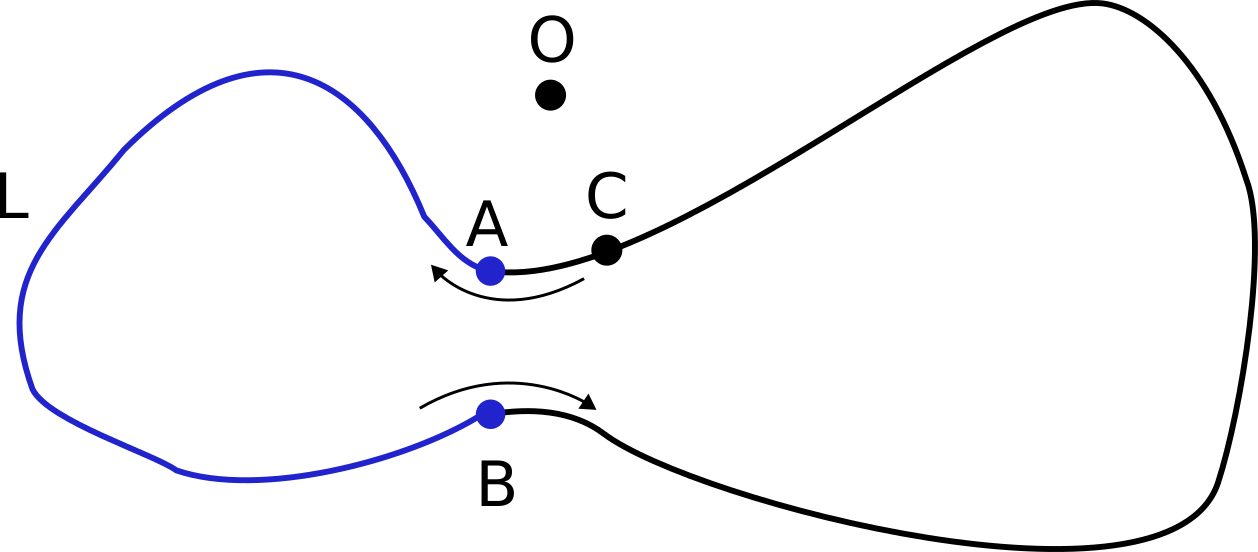
\includegraphics[width=0.9\linewidth]{images/parameter.png}
  \caption[]{A dumbbell-like boundary of a pore. Points $A$ and $B$ form a
    bottleneck while points $A$ and $C$ do not. This can seen by a relative
    position of the point $O$ while traversing the boundary
    counter-clockwise. Namely, it's on the left side when crossing $A$ but on
    the right side when crossing $B$. When crossing $A$ and $C$, the relative
    position of $O$ does not change. The parameter $p_{AB}$ is equal to the
    distance between $A$ and $B$ divided by length of the blue contour $L$.}
  \label{fig:parameter}
\end{figure}

Although a guaranteed upper bound for $p$ is 1, it's reachable only for
degenerate shapes in the form of line segments. The biggest value for
non-degenerate shapes is reached for a disk and equals to $2/\pi$. Similarly, an
ellipse defined as
\begin{equation*}
  \frac{x^2}{a^2} + \frac{y^2}{b^2} = 1
\end{equation*}
has the biggest known value of $p$ from all shapes with elongation $E = a / b$
(suppose $a \le b$). Using Ramanujan's formula for the perimeter of an ellipse
we get
\begin{equation*}
  p \le p_{ellipse} = \frac{2a}{P/2} \approx \frac{4E}{\pi[3(1+E) - \sqrt{(3E+1)(E+3)}]}
\end{equation*}
where $P$ is a perimeter of the ellipse. By dividing $p$ by $p_{ellipse}$ we
obtain an improved pore shape parameter $P$:
\begin{equation*}
  P = \frac{\pi p [3(1+E) - \sqrt{(3E+1)(E+3)}]}{4E}
\end{equation*}

Substituting \cref{eq:pre-awesomeness} and \cref{eq:intro} we get a new pore
shape parameter we call ``\highlight{awesomeness}'':
\begin{equation}
  \begin{aligned}
    P &= \frac{\pi [3(1+E) - \sqrt{(3E+1)(E+3)}]}{4E} \times \\
    & \times \inf \{\frac{\rho_{AB}}{L_{AB}} \ \forall (A, B) \in B^2\}
  \end{aligned}
  \label{eq:awesomeness}
\end{equation}
where, again, $E$ and $B$ are the elongation the boundary of the pore,
$\rho_{AB}$ is the Euclidean distance between points $A$ and $B$ and $L_{AB}$ is
the length of a path (the shortest one) between $A$ and $B$ along the boundary.

\section{Computational algorithm}
\label{seq:alg}
Our algorithm for calculating \highlight{awesomeness} is quite simple. It
assumes that an image of a pore is made with sufficient resolution, so we can
use boundary pixels without any additional processing. The main algorithm
consists of three parts and is shown in \cref{alg:main}.
\begin{algorithm}[H]
  \caption{Algorithm for computation of \highlight{awesomeness} of a pore.}
  \label{alg:main}
  \begin{algorithmic}[1]
    \Procedure{\texttt{awesomeness}}{\texttt{img}}
    \State \texttt{bs $\gets$ boundary(img)}
    \Comment Construct a list of boundary points (\cref{alg:extraction}).
    \State \texttt{\%bs $\gets$ sort(bs)}
    \Comment Sort points as described in \cref{alg:sort}.
    \State \textbf{return} \texttt{c $\cdot$ pmin(\%bs)}
    \Comment The final step is in \cref{alg:pmin}. \texttt{c} is the fraction in
    \cref{eq:awesomeness}.
    \EndProcedure
  \end{algorithmic}
\end{algorithm}

The first step extracts a list of boundary points from an image of a pore, the
second step sorts them in the order descried later and the third and the last
step minimizes $p_{AB}$ parameter for each pair of points $(A, B)$ which lie on
the boundary.

Suppose the boundary is defined by a parameteric equation
\begin{equation*}
  \left\{
  \begin{aligned}
    x &= f(t) \\
    y &= g(t)
  \end{aligned}
  \right.
\end{equation*}
or, using a shorter notation,
$B = \begin{pmatrix} x_B \\ y_B \end{pmatrix} = \begin{pmatrix} f \\ g \end{pmatrix}(t)$
Suppose, you have two points: $B_1 = \begin{pmatrix} f \\ g \end{pmatrix}(t_1)$
and $B_2 = \begin{pmatrix} f \\ g \end{pmatrix}(t_2)$. The sorting in the step 2
implies that if $t_1 < t_2$, the point $B_1$ must appear before $B_2$ in
\texttt{\%bs}.

In the following algorithms we will use a notion of single linked lists (or
simply lists). A list of elements of type \texttt{a} can be defined using the
following data type with two constructors, \texttt{[]} and \texttt{(:)}:
\begin{verbatim}
data List a = [] | a:(List a)
\end{verbatim}
The first constructor creates an empty list and the second attaches an element
of type \texttt{a} to the list of elements of type \texttt{a}. Sometimes we will
use conventional functions for working with lists such as \texttt{head},
\texttt{tail}, \texttt{map}, \texttt{foldl} and so on.

The algorithm for boundary extraction is shown in \cref{alg:extraction}.
\begin{algorithm}[H]
  \caption{Algorithm for boundary extraction. Takes an image of a pore and
    returns a list of points (indices) which belong to the boundary. It assumes,
  that pore pixels have a value 1 and background pixels have a value 0.}
  \label{alg:extraction}
  \begin{algorithmic}[1]
    \Procedure{\texttt{boundary}}{\texttt{img}}
    \Procedure{\texttt{boundaryp}}{\texttt{index}}
    \State \textbf{return} true if there are background pixels to the left,
    right, up or down from the pixel with this index, false otherwise.
    \EndProcedure
    \Procedure{\texttt{accumulate}}{\texttt{acc, index}}
    \If{\texttt{img[index] = 1} $\wedge$ \texttt{boundaryp(index)}}
    \State \textbf{return} \texttt{index:acc}
    \Else
    \State \textbf{return} \texttt{acc}
    \EndIf
    \EndProcedure
    \State \textbf{return} \texttt{foldl accumulate [] all\_indices(img)}
    \EndProcedure
  \end{algorithmic}
\end{algorithm}

Sorting the boundary points can be done by ensuring that every two consecutive
points have Chebyshev distance equal to 1. This is done by making a list which
contains some (maybe random) point belonging to the boundary and successive
addition of neighbor points (relative to the head of that list) to the list. It
may be that all neighbors must be tried to successfully construct the sorted
list.

As a heuristic, we maintain a list of seen neighbors, that is, for every point
added to the sorted list we obtain all its neighbors and add them to a separate
list. When a point is added to the sorted list, it is removed from that
list. Before adding any point we consult this list of neighbors to ensure that
there is no point which is farther than 1 from the point on the head of the
sorted list. If this is not so, we give up with the current sorted list and try
to find another list instead.

The final remark is that in order to find neighbors of a point we either have to
build a metric tree (like BK-tree) or keep one extra bit array to mark boundary
points and provide a way to do quick searches for neighbors of some arbitrary
point. A complete algorithm is \cref{alg:sort} where BK-trees are used.
\begin{algorithm}[H]
  \caption{Algorithm for sorting a list of boundary points.}
  \label{alg:sort}
  \begin{algorithmic}[1]
    \Procedure{\texttt{sort}}{\texttt{points}}
    \State \texttt{start $\gets$ head(points)}
    \State \texttt{tree $\gets$ bk\_tree(tail(points))}
    \Procedure{\texttt{go}}{\texttt{sorted, neighbors, tree}}
    \Comment \texttt{sorted} contains a list of sorted boundary points,
    \texttt{neighbors} is an additional list of seen neighbors, \texttt{tree} is
    a BK-tree of unsorted points.
    \If{\texttt{tree\_empty\_p(tree)}}
    \State \textbf{return} \texttt{sorted}
    \Comment No more unsorted points, we are finished.
    \EndIf
    \State \texttt{last $\gets$ head(sorted)}
    \Procedure{\texttt{check\_dist}}{\texttt{point}}
    \State \textbf{return} \texttt{cheb\_dist(last, point) = 1}
    \EndProcedure
    \If{\texttt{notevery(check\_dist, neighbors)}}
    \State \textbf{return} \texttt{[]}
    \Comment We have failed, try to sort another way
    \EndIf
    \State \texttt{ns $\gets$ bk\_tree\_search(tree, last, 1)}
    \Comment Search all points which have Chebyshev distance to \texttt{last} no
    more than 1.
    \State \texttt{\%neighbors $\gets$ tail(sorted) = [] ? [] : union(neighbors, ns)}
    \Comment If we have only one point in the sorted list, do not keep the
    neighbors.
    \Procedure{\texttt{\%go}}{\texttt{neighbor}}
    \State \texttt{\%sorted $\gets$ neighbor:sorted}
    \State \texttt{\%\%neighbors $\gets$ remove(neighbor, \%neighbors)}
    \State \texttt{\%tree $\gets$ bk\_tree\_remove(tree, neighbor)}
    \State \textbf{return} \texttt{go(\%sorted, \%\%neighbors, \%tree)}
    \EndProcedure
    \State \texttt{sorted $\gets$ map(\%go, ns)}
    \State \textbf{return} The first non-empty list from \texttt{sorted}, if
    any. Otherwise return \texttt{[]}.
    \EndProcedure
    \State \textbf{return} \texttt{go([start], [], tree)}
    \EndProcedure
  \end{algorithmic}
\end{algorithm}

The \cref{alg:sort} serves two purposes: not only it sorts boundary points, it
also checks the boundary for correctness. If boundary points in the unsorted
list do not represent a simple closed curve (like on \cref{fig:good-and-bad}),
\texttt{sort} will return an empty list.
\begin{figure}[tp]
  \centering
  \subfigure[A good boundary]{
    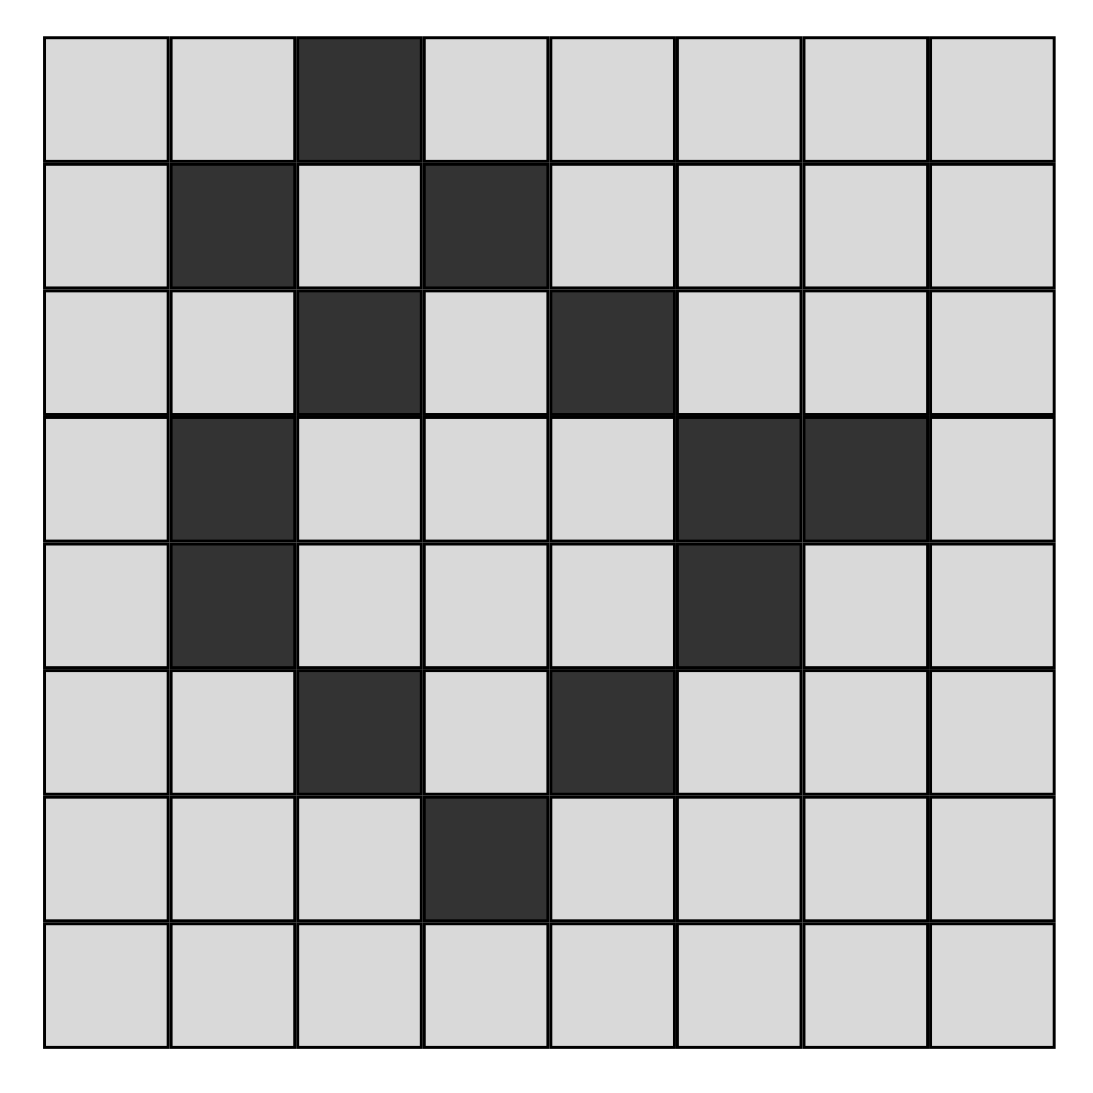
\includegraphics[width=0.4\linewidth]{images/good.png}}
  \subfigure[Points do not represent a simple curve (one point is crossed
    twice)]{
    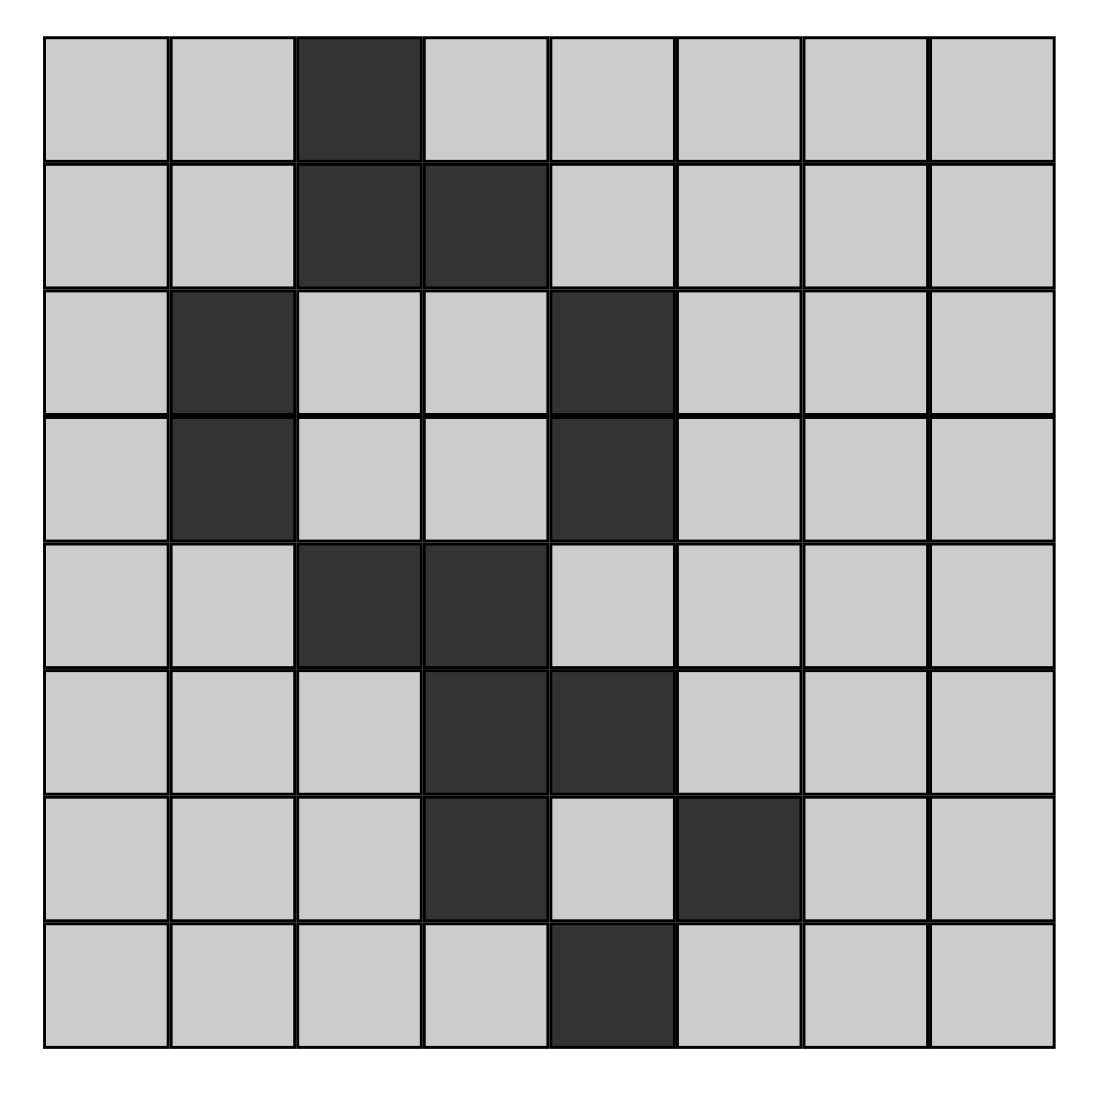
\includegraphics[width=0.4\linewidth]{images/bad.png}}
  \vskip\baselineskip
  \subfigure[Some points are crossed twice]{
    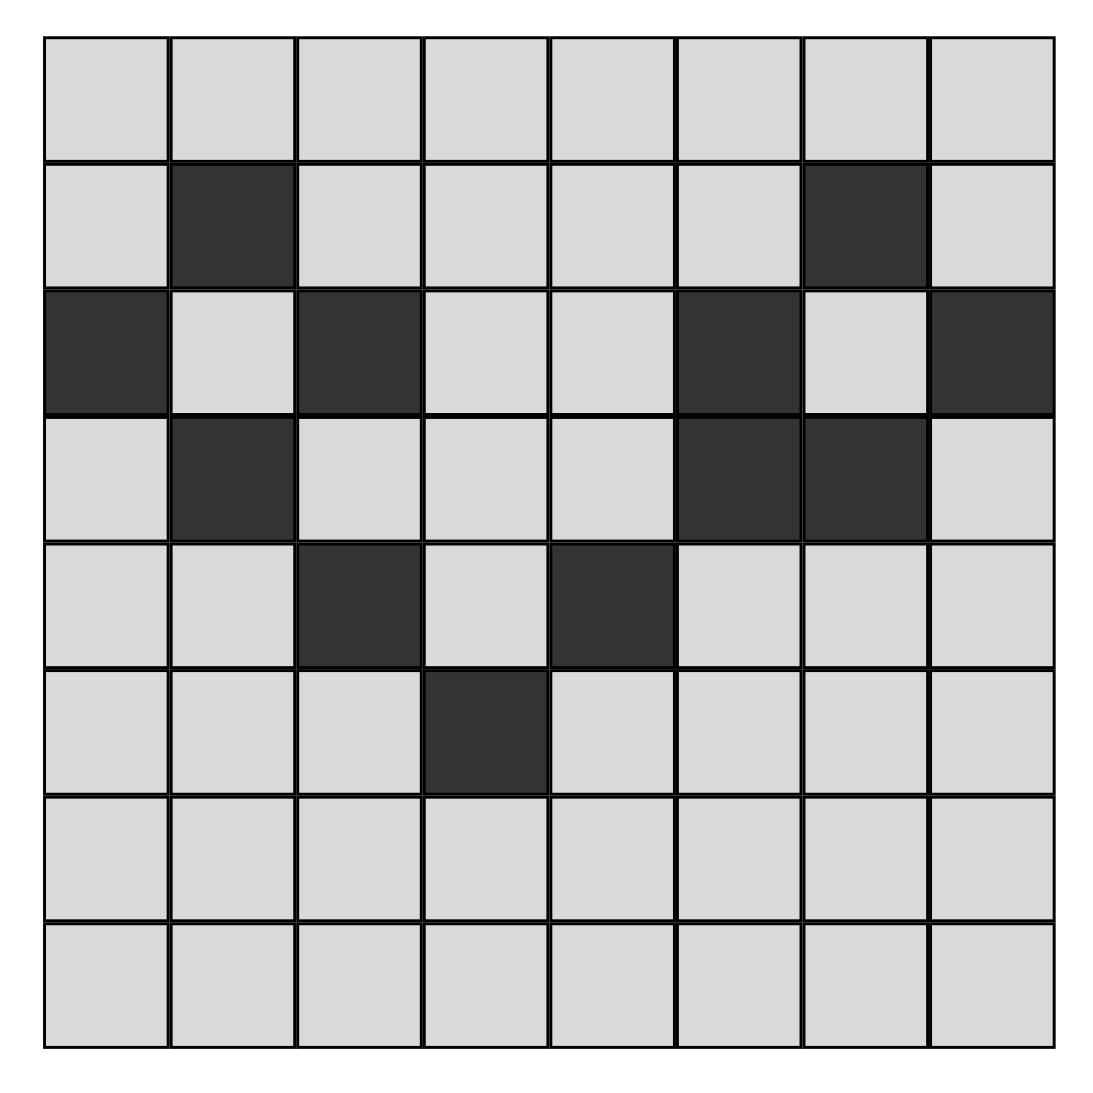
\includegraphics[width=0.4\linewidth]{images/bad2.png}}
  \subfigure[Points do not represent a closed curve]{
    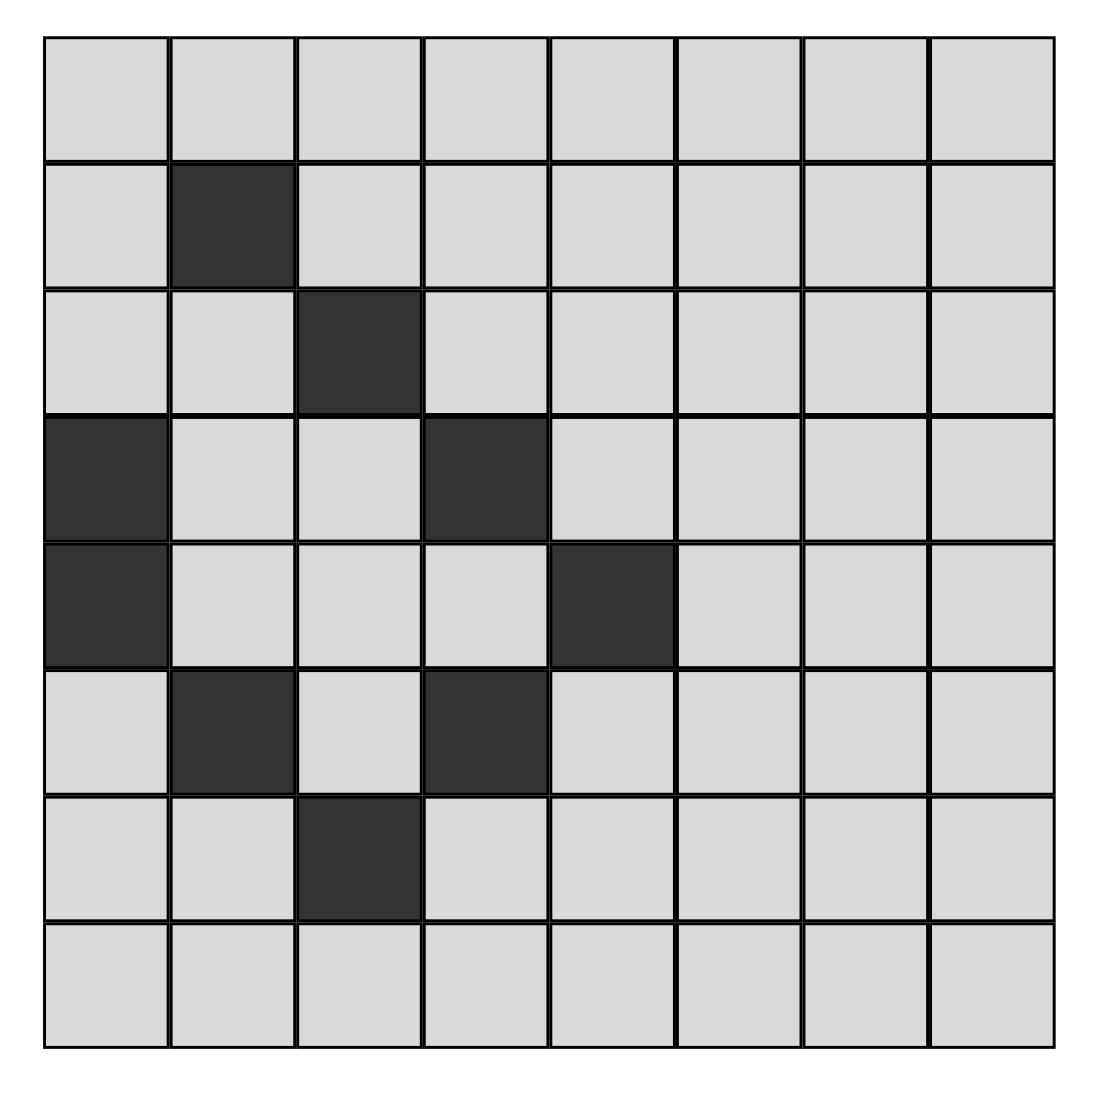
\includegraphics[width=0.4\linewidth]{images/bad3.png}}
  \caption[]{A good set of boundary points and three examples of inacceptable
    boundary discarded by \texttt{sort}.}
  \label{fig:good-and-bad}
\end{figure}

Finaly, the function \texttt{pmin} is described in \cref{alg:pmin}. This
algorithms assumes that there are enough boundary points in an image. If, for
example, an image is taken with bad resolution (i.e. pores consist only of a few
pixels) some quality improving techniques must be applied first. It also
exploits the commutative property $p_{AB} = p_{BA}$.
\begin{algorithm}[H]
  \caption{The last step of the algorithm for awesomeness: the function \texttt{pmin}.}
  \label{alg:pmin}
  \begin{algorithmic}[1]
    \Procedure{\texttt{pairwise\_distances}}{\texttt{points}}
    \State \textbf{return} \texttt{map(dist, points, tail(points))}
    \Comment Return the Euclidean distance between $i$-th and $i+1$-th
    points. The function \texttt{dist} calculates the distance between two
    points.
    \EndProcedure
    \Procedure{\texttt{perimeter}}{\texttt{points}}
    \State \texttt{p1 $\gets$ foldl((+), 0, pairwise\_distances(points))}
    \State \texttt{p2 $\gets$ dist(head(points), last(points))}
    \State \textbf{return} \texttt{p1 + p2}
    \EndProcedure
    \Procedure{\texttt{minimize\_on\_head}}{\texttt{acc, p, points}}
    \Comment \texttt{acc} is the best (minimal) parameter found so far,
    \texttt{p} is a perimeter of the boundary.
    \Procedure{\texttt{go}}{\texttt{acc, x}}
    \State \texttt{(point, boundary\_dist) $\gets$ x}
    \State \texttt{awesomeness $\gets$ dist(point, head(points)) /
      min(boundary\_dist, p - boundary\_dist)}
    \State \textbf{return} \texttt{min(acc, awesomeness)}
    \EndProcedure
    \State \texttt{ds $\gets$ scanl((+), 0, pairwise\_distances(points))}
    \State \texttt{tmp $\gets$ zip(tail(points), tail(ds))}
    \State \textbf{return} \texttt{foldl(go, acc, tmp)}
    \EndProcedure
    \Procedure{\texttt{pmin}}{\texttt{points}}
    \State \texttt{p $\gets$ perimeter(points)}
    \Procedure{\texttt{go}}{\texttt{acc, points}}
    \State \textbf{return} \texttt{minimize\_on\_head(acc, p, points)}
    \EndProcedure
    \State \textbf{return} \texttt{foldl(go, +infinity, points)}
    \EndProcedure
  \end{algorithmic}
\end{algorithm}
If \texttt{sort} cannot sort boundary points, \texttt{pmin} will return
\texttt{+infinity}.

\section{Results}
We computed \highlight{awesomeness} for 4000 synthetically generated images with
dimensions $1000 \times 1000$ pixels (1000 images from 4 different
datasets). The datasets have the following properties:
\begin{itemize}
\item \texttt{normal}: ``Normal'' pores with convexity $0.5-0.8$.
\item \texttt{mnist}: Pores which resemble digits (still being 1-connected).
\item \texttt{thin}: Pores with low convexity ($< 0.5$) which resemble thin
  stripes.
\item \texttt{mostlyconvex}: Pores with convexity close to $1$.
\end{itemize}
Figure \ref{fig:pores} depicts a pore from each dataset.
\begin{figure}
  \centering
  \subfigure[\texttt{normal}]{
    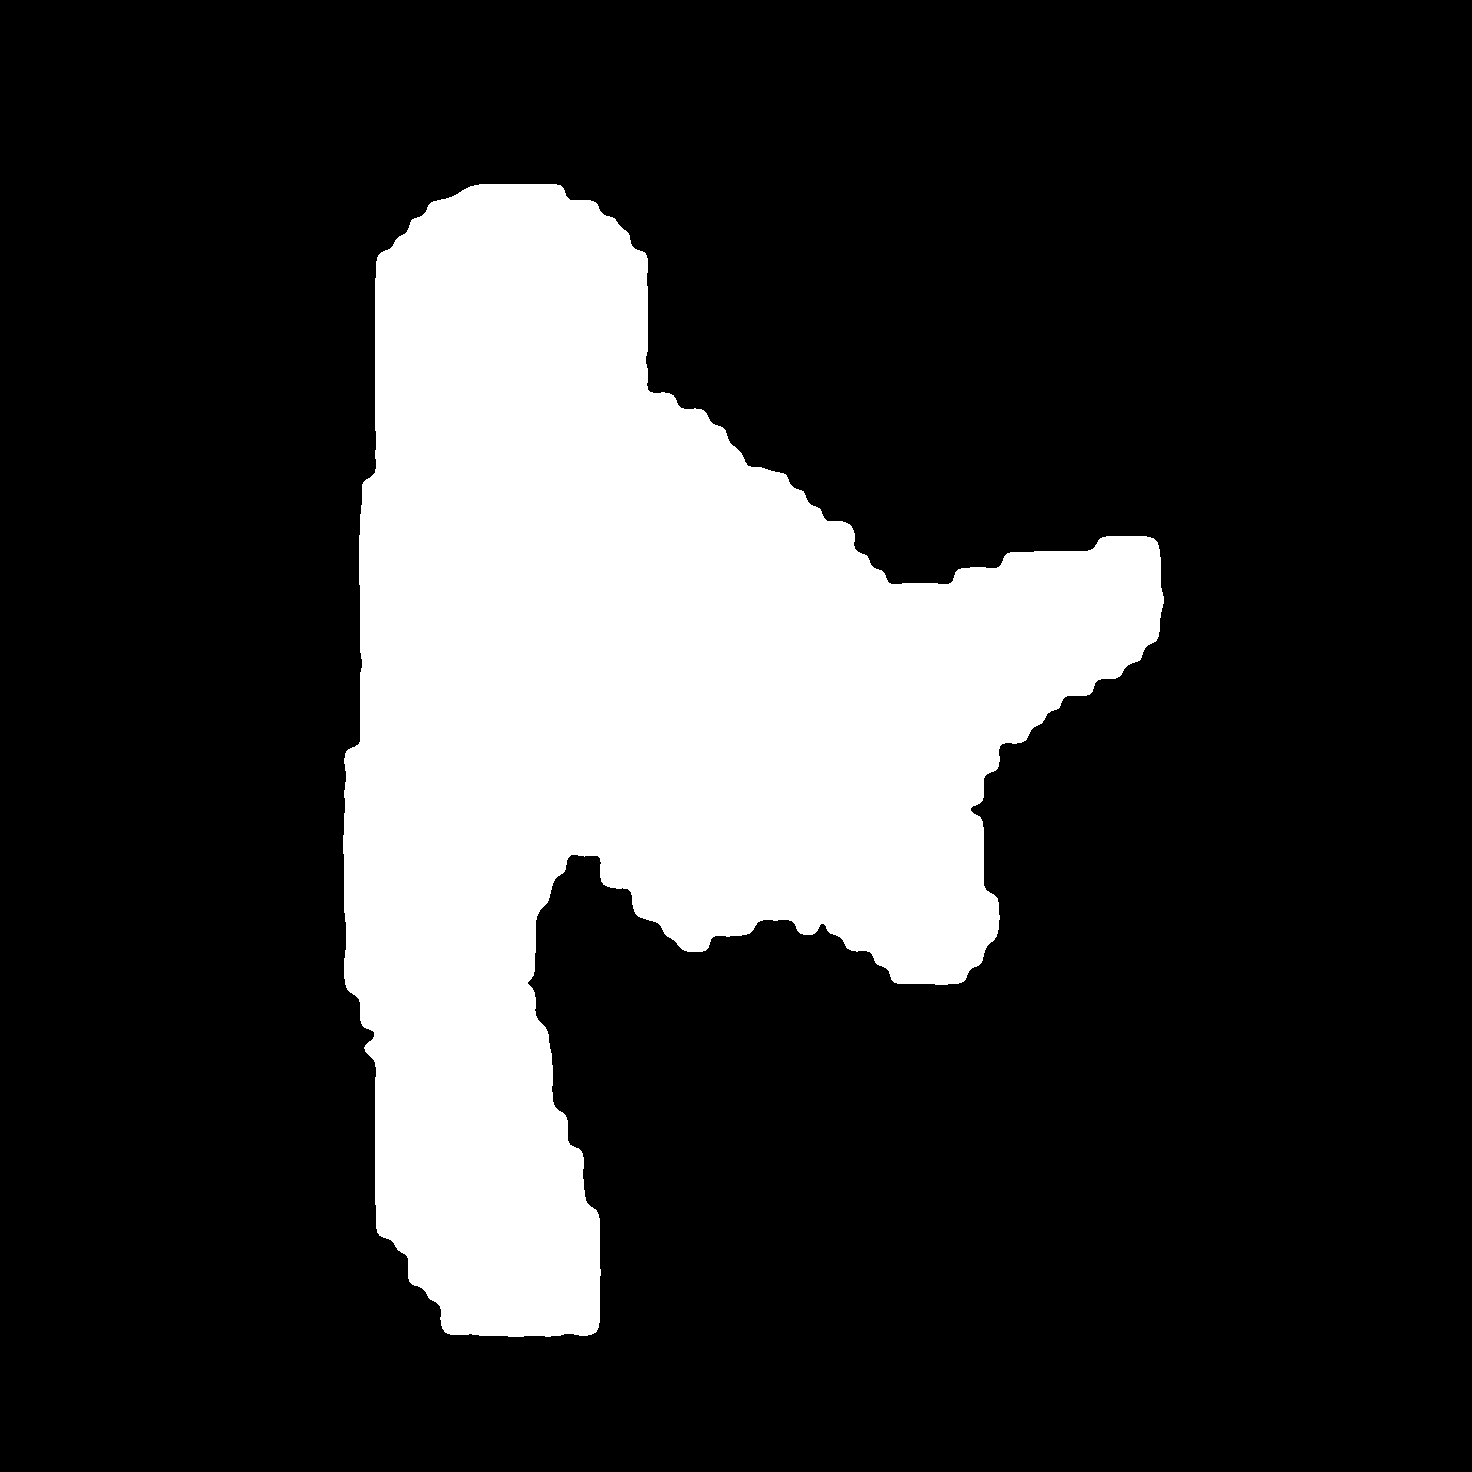
\includegraphics[width=0.4\linewidth,frame]{images/normal.png}}
  \subfigure[\texttt{thin}]{
    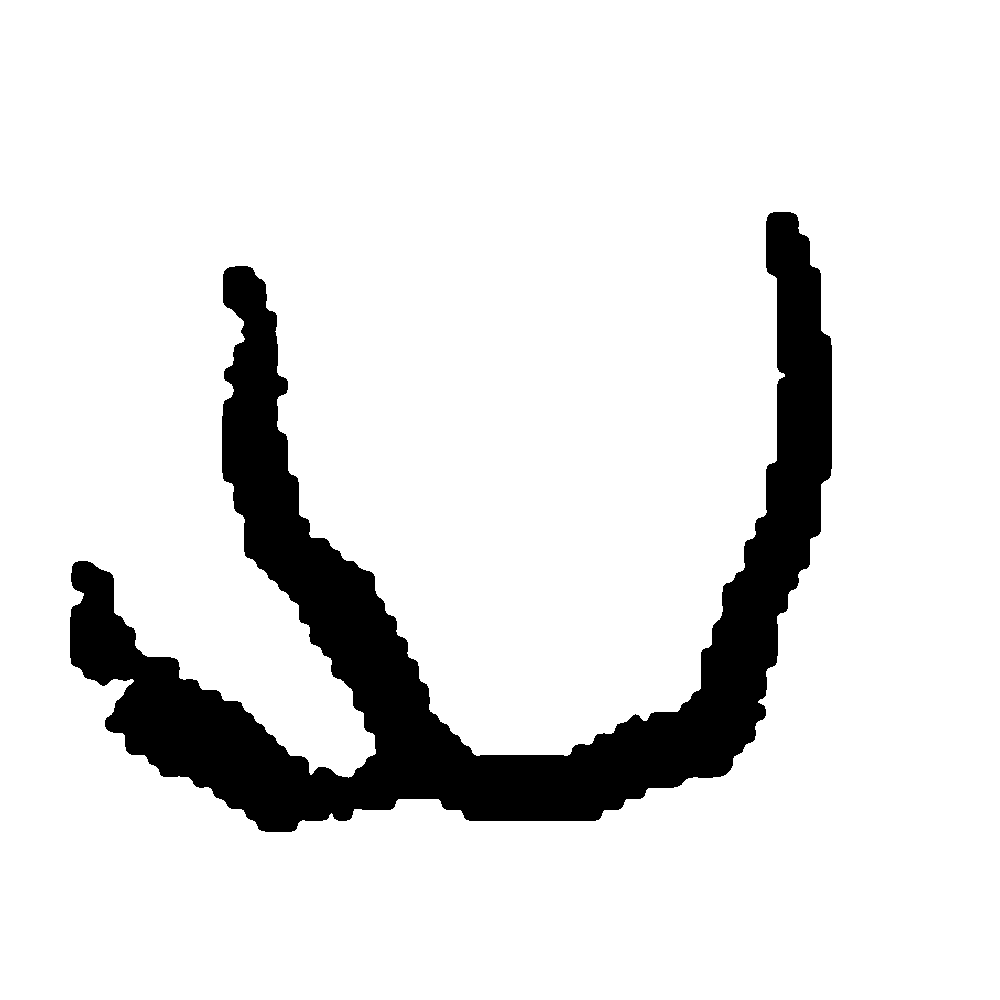
\includegraphics[width=0.4\linewidth,frame]{images/thin.png}}
  \vskip\baselineskip
  \subfigure[\texttt{mnist}]{
    
\includegraphics[width=0.4\linewidth,frame]{images/mnist.png}}
  \subfigure[\texttt{mostlyconvex}]{
    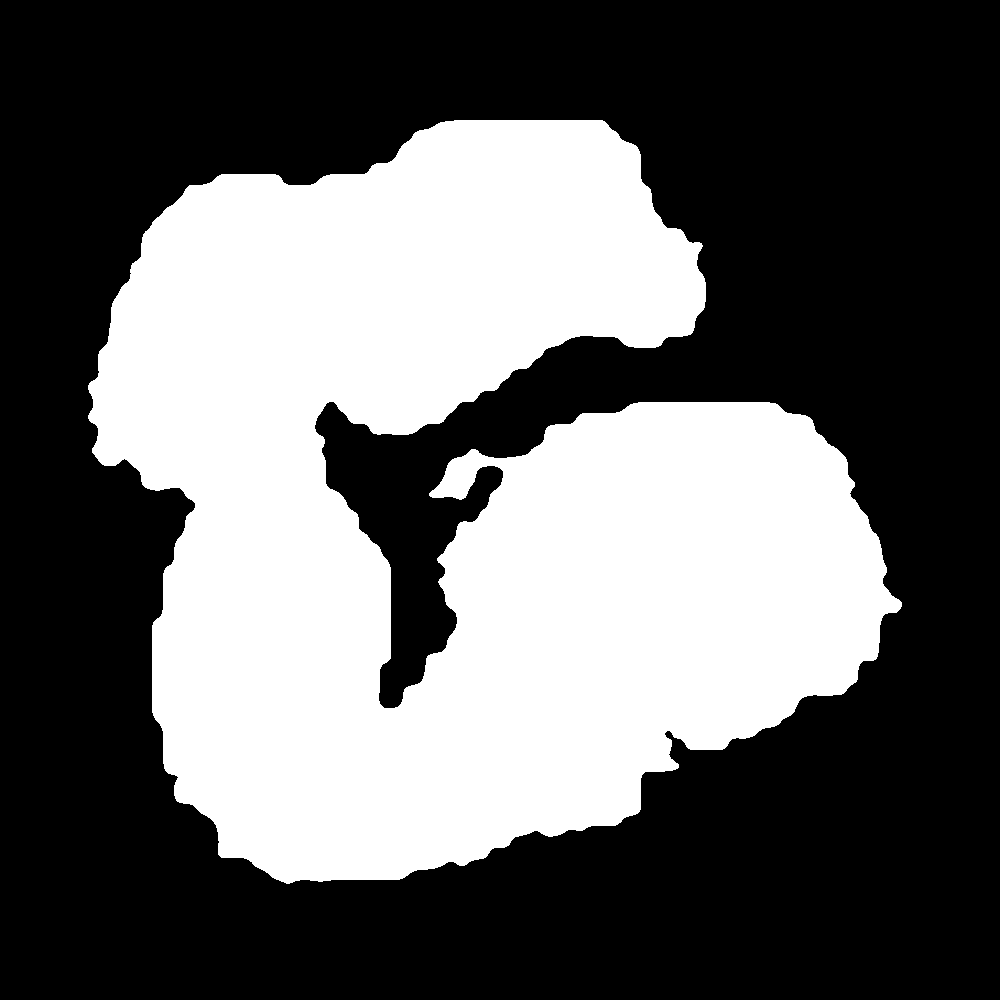
\includegraphics[width=0.4\linewidth,frame]{images/mostlyconvex.png}}
  \caption[]{One pore from each dataset used for calculation of
    \texttt{awesomeness}.}
  \label{fig:pores}
\end{figure}

Summarly 3901 images out of 4000 (97.5\%) were good enough for \texttt{sort} to
sort boundary points in pores. For these images we also computed commonly used
convexity and elongation parameters. On \cref{fig:cae-space} each pore is
represented as a dot in convexity-elongation-\highlight{awesomeness} (CEA)
space.
\begin{figure*}
  \centering
  \subfigure[Convexity-elongation-\highlight{awesomeness} space]{
    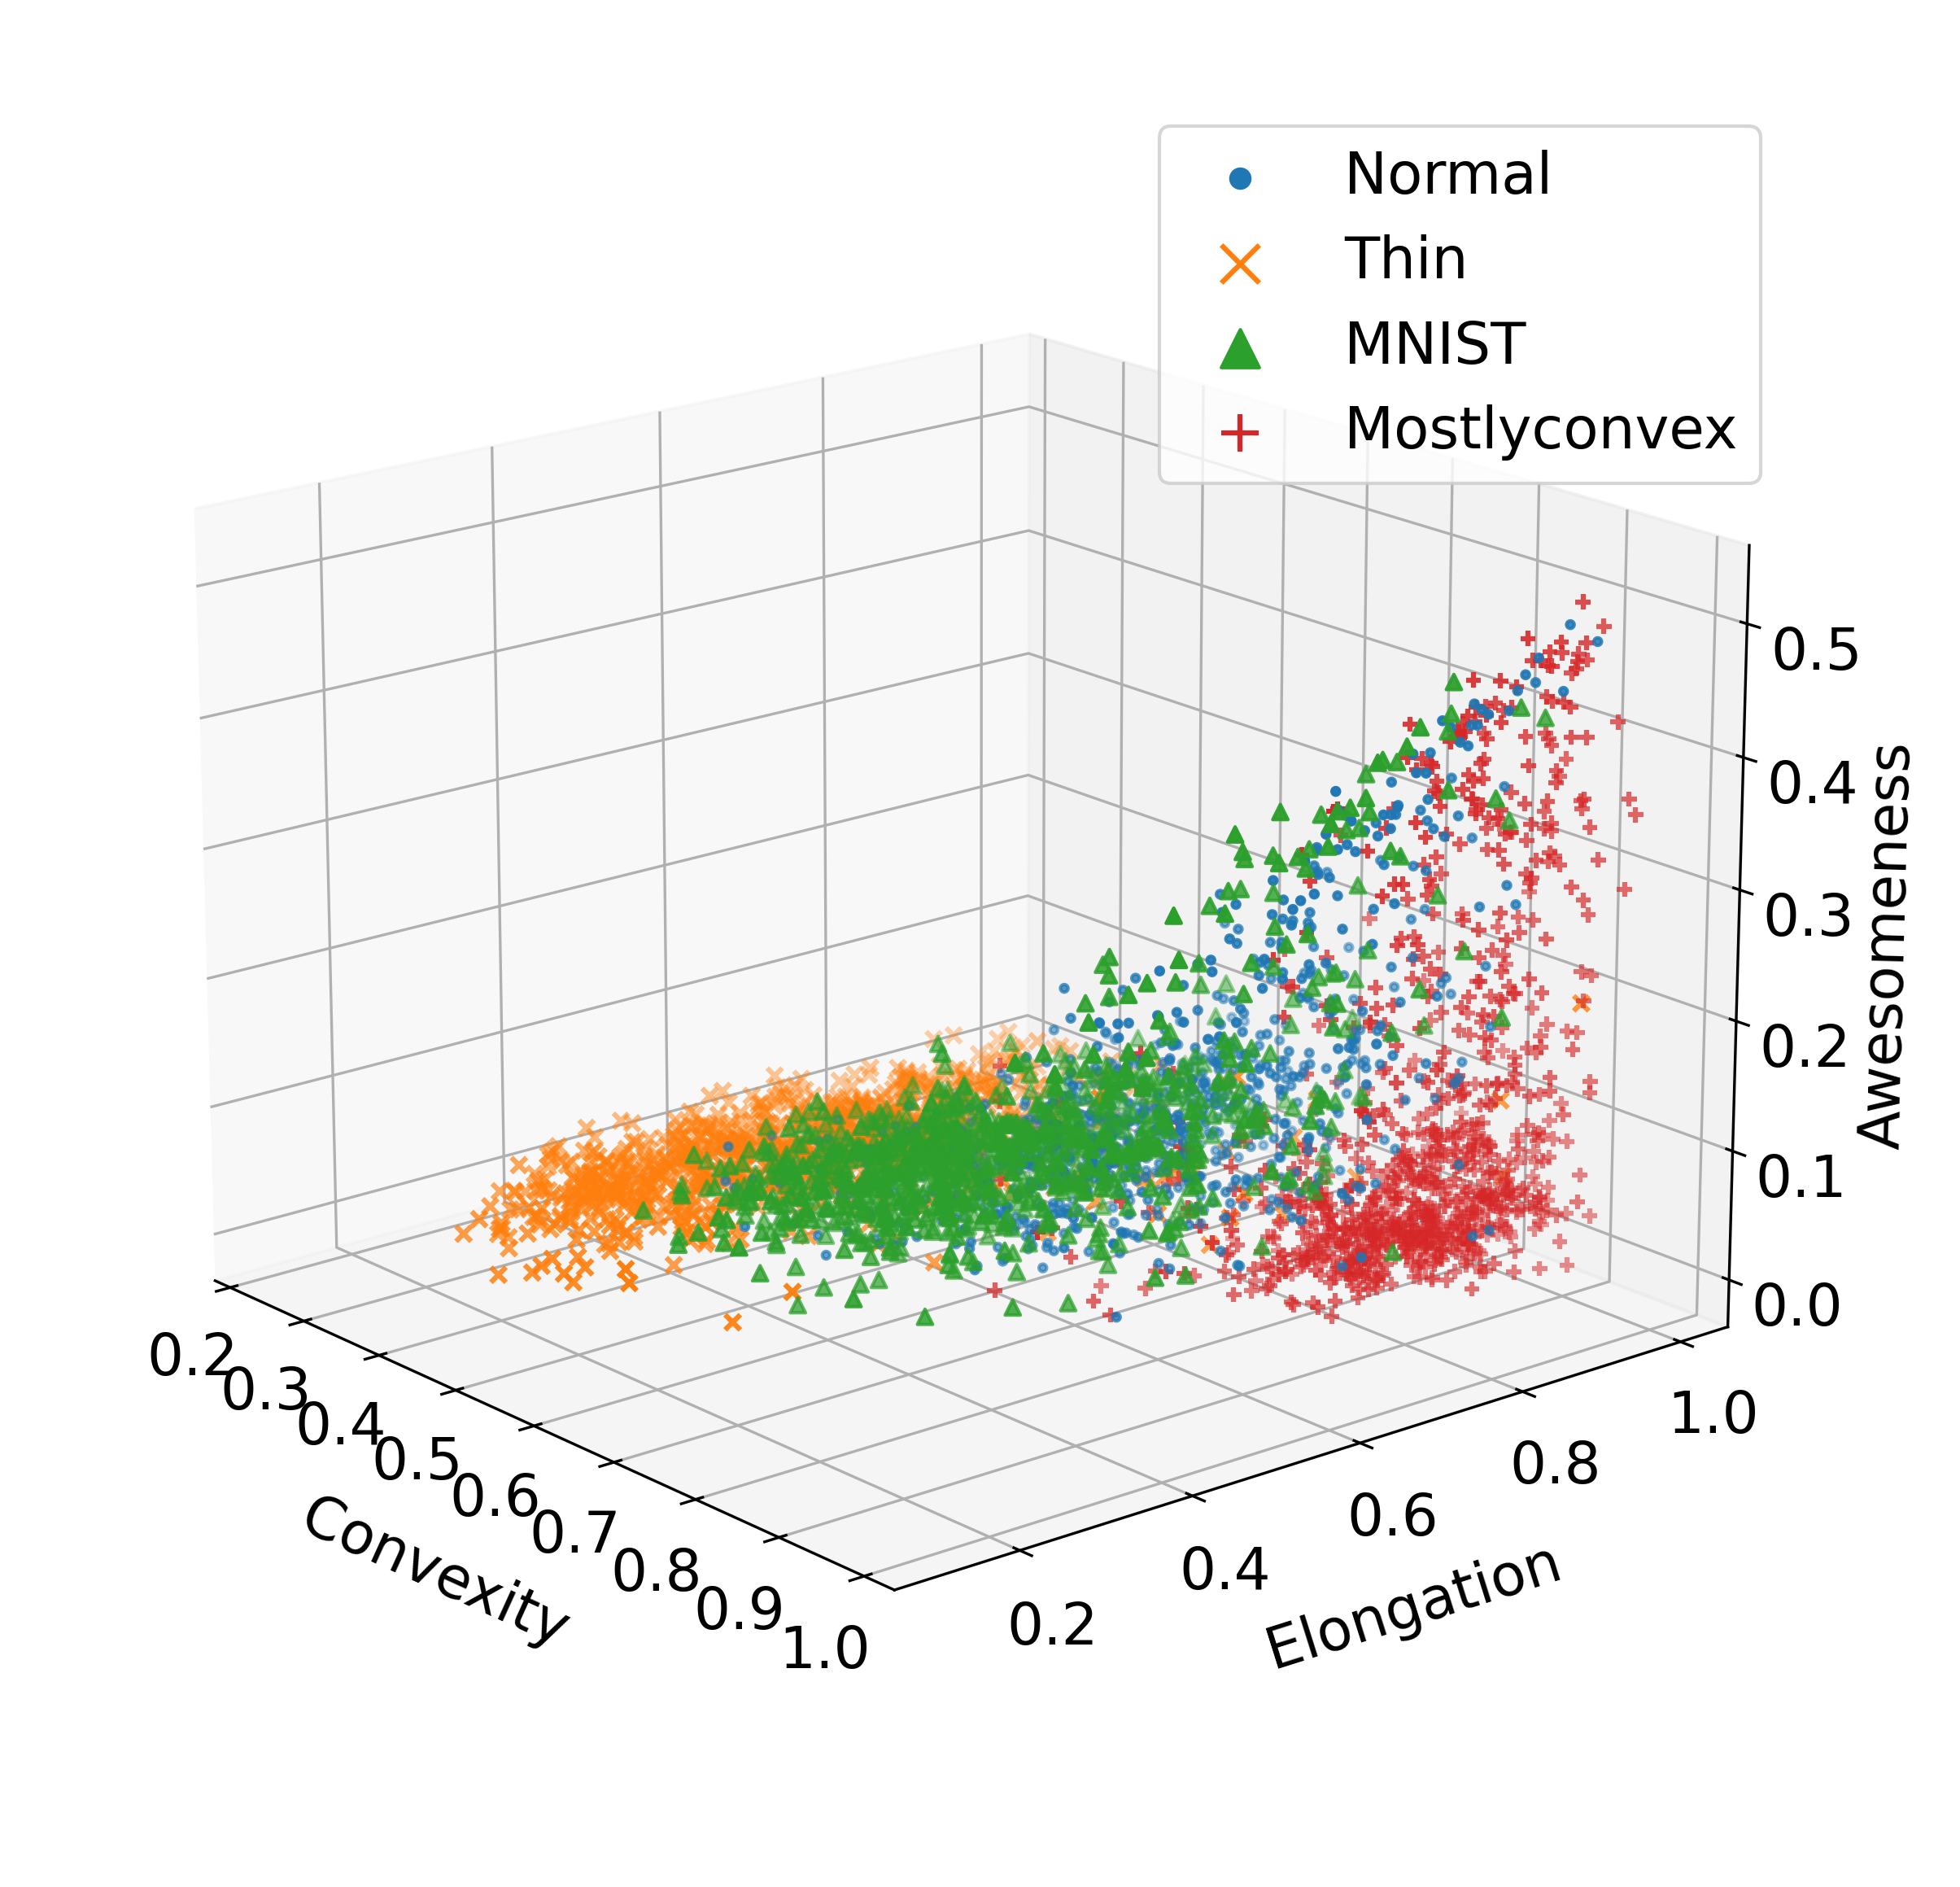
\includegraphics[width=0.4\linewidth]{images/cae.png}
    \label{fig:cae-space}}
  \hfill
  \subfigure[Convexity-elongation-roundness space]{
    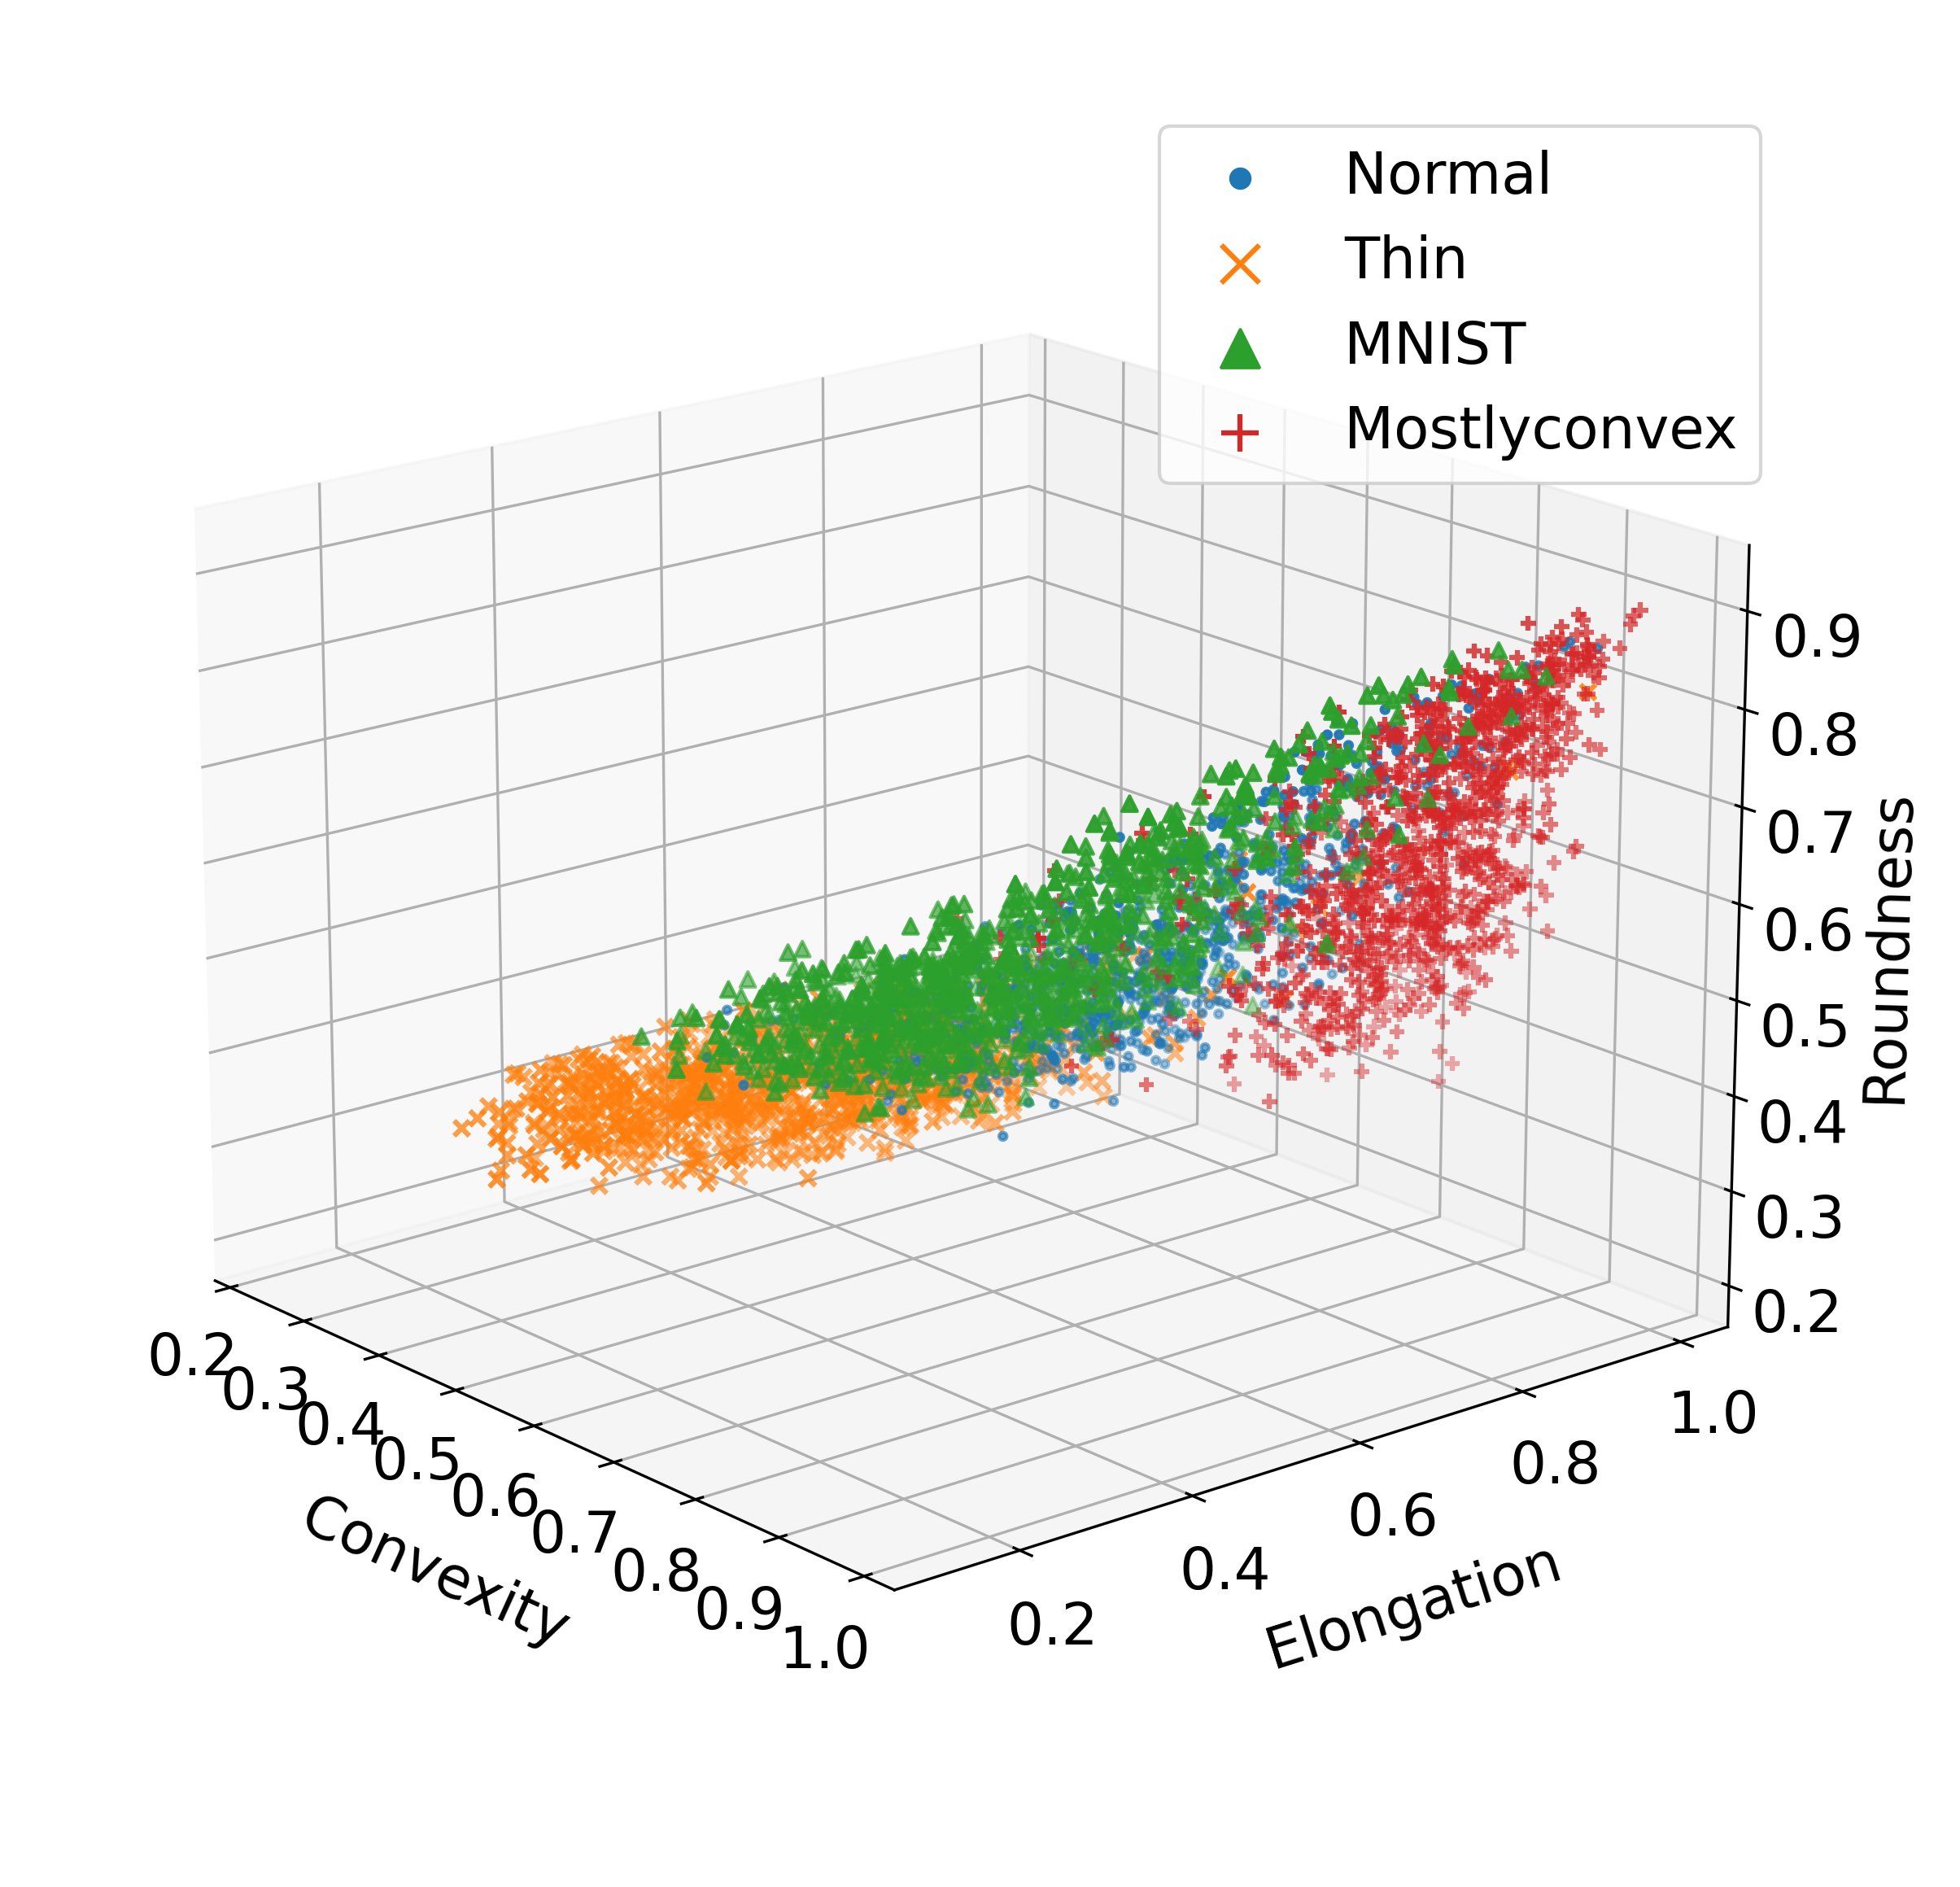
\includegraphics[width=0.4\linewidth]{images/cer.png}
    \label{fig:cer-space}}
  \vskip\baselineskip
  \subfigure[Elongation-\highlight{Correlated awesomeness} space]{
    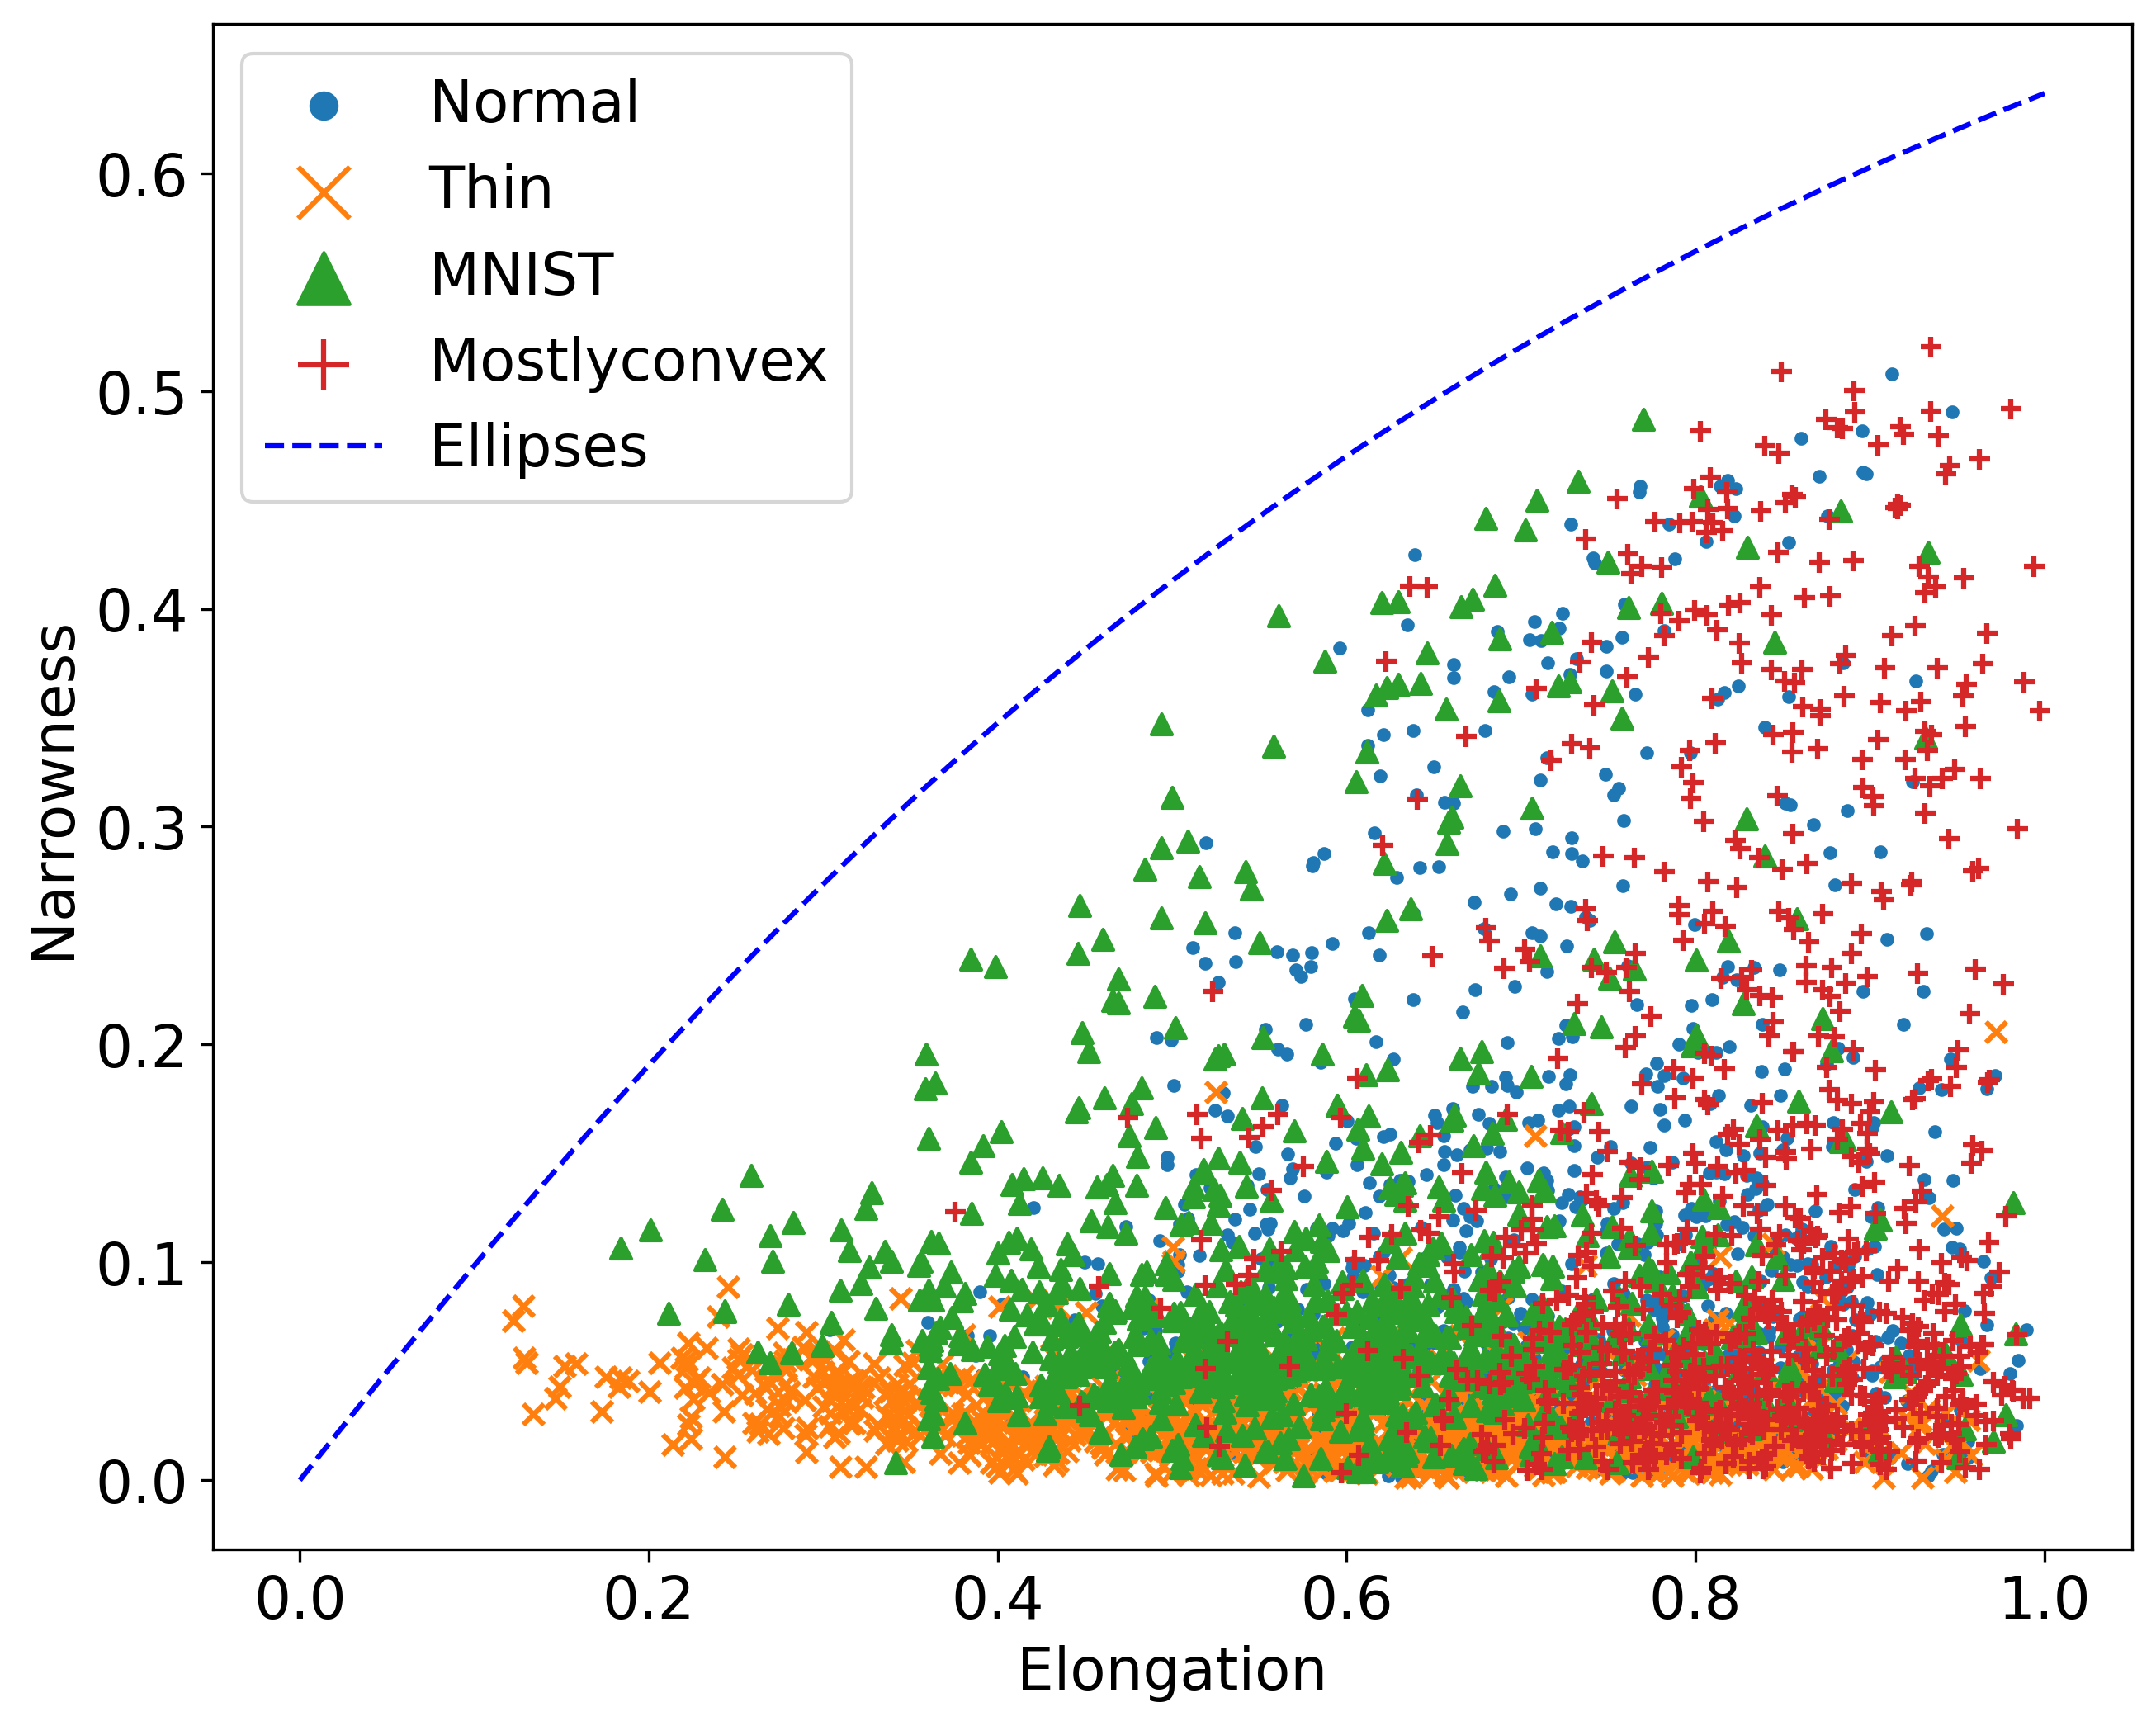
\includegraphics[width=0.4\linewidth]{images/ae.png}
    \label{fig:ae-space}}
  \caption[]{Synthetically generated pores shown as points in different
    parameter spaces.}
  \label{fig:parameter-spaces}
\end{figure*}

It can be seen that if a pore has low convexity ($< 0.6$)
\highlight{awesomeness} adds no information to the pore's descriptors because it
stays relatively low for all pores. When, however, the convexity is high it adds
a new dimension to the parameter space.

Another common parameter for describing pore shapes is roundness. Figure
\ref{fig:cer-space} features convexity-elongation-roundness (CER) space.
It can be seen that roundness-convexity correlation is bigger than
awesomeness-convexity correlation. All correlation values are in
\cref{tab:correlations}.

On \cref{fig:ae-space} pores are shown in $p-E$ space where $p$ is a
``correlated'' \highlight{awesomeness} parameter \cref{eq:pre-awesomeness}. It
shows that our assumption on the maximal value of \highlight{awesomeness} is
correct indeed.

\begin{table*}[!htp]
  \centering
  \begin{tabular}{|c|c|c|c|c|}
    \hline
    & Awesomeness & Elongation & Convexity & Roundness \\
    \hline
    Awesomeness & 1 & 0.049 & 0.557 & 0.745 \\
    \hline
    Elongation & & 1 & 0.457 & 0.355 \\
    \hline
    Convexity &&& 1 & 0.922 \\
    \hline
    Roundness &&&& 1 \\
    \hline
  \end{tabular}
  \caption{Correlation between shape describing parameters.}
  \label{tab:correlations}
\end{table*}

To test abilities of the awesomeness parameter we now divide our pores in groups
with different convexity. The first group has pores with convexity $0.55 \le C < 0.65$,
the second -- $0.65 \le C < 0.75$, the third -- $0.75 \le C < 0.85$ and the fourth
-- $0.85 \le C < 0.95$. Five images with the biggest awesomeness and five images
with the smallest awesomeness from each group are shown on
\cref{fig:convexity-groups-score}. It can be clearly seen that pores with higher
values of \highlight{awesomeness} are more ``solid'' and more finely
clusterized.

For comparison, we do the same sorting across groups for roundness
parameter. The results are on
\cref{fig:convexity-groups-roundness}. Well-clusterized pores have the biggest
roundness for convexity $C > 0.8$. For lower convexity, however, even pores with
the biggest roundness in the group are also underclusterized while
\highlight{awesomeness} parameter is capable of separating well-clusterized and
underclusterized pores.
\begin{figure*}
  \centering
  \subfigure[$0.55 \le C < 0.65$]{
    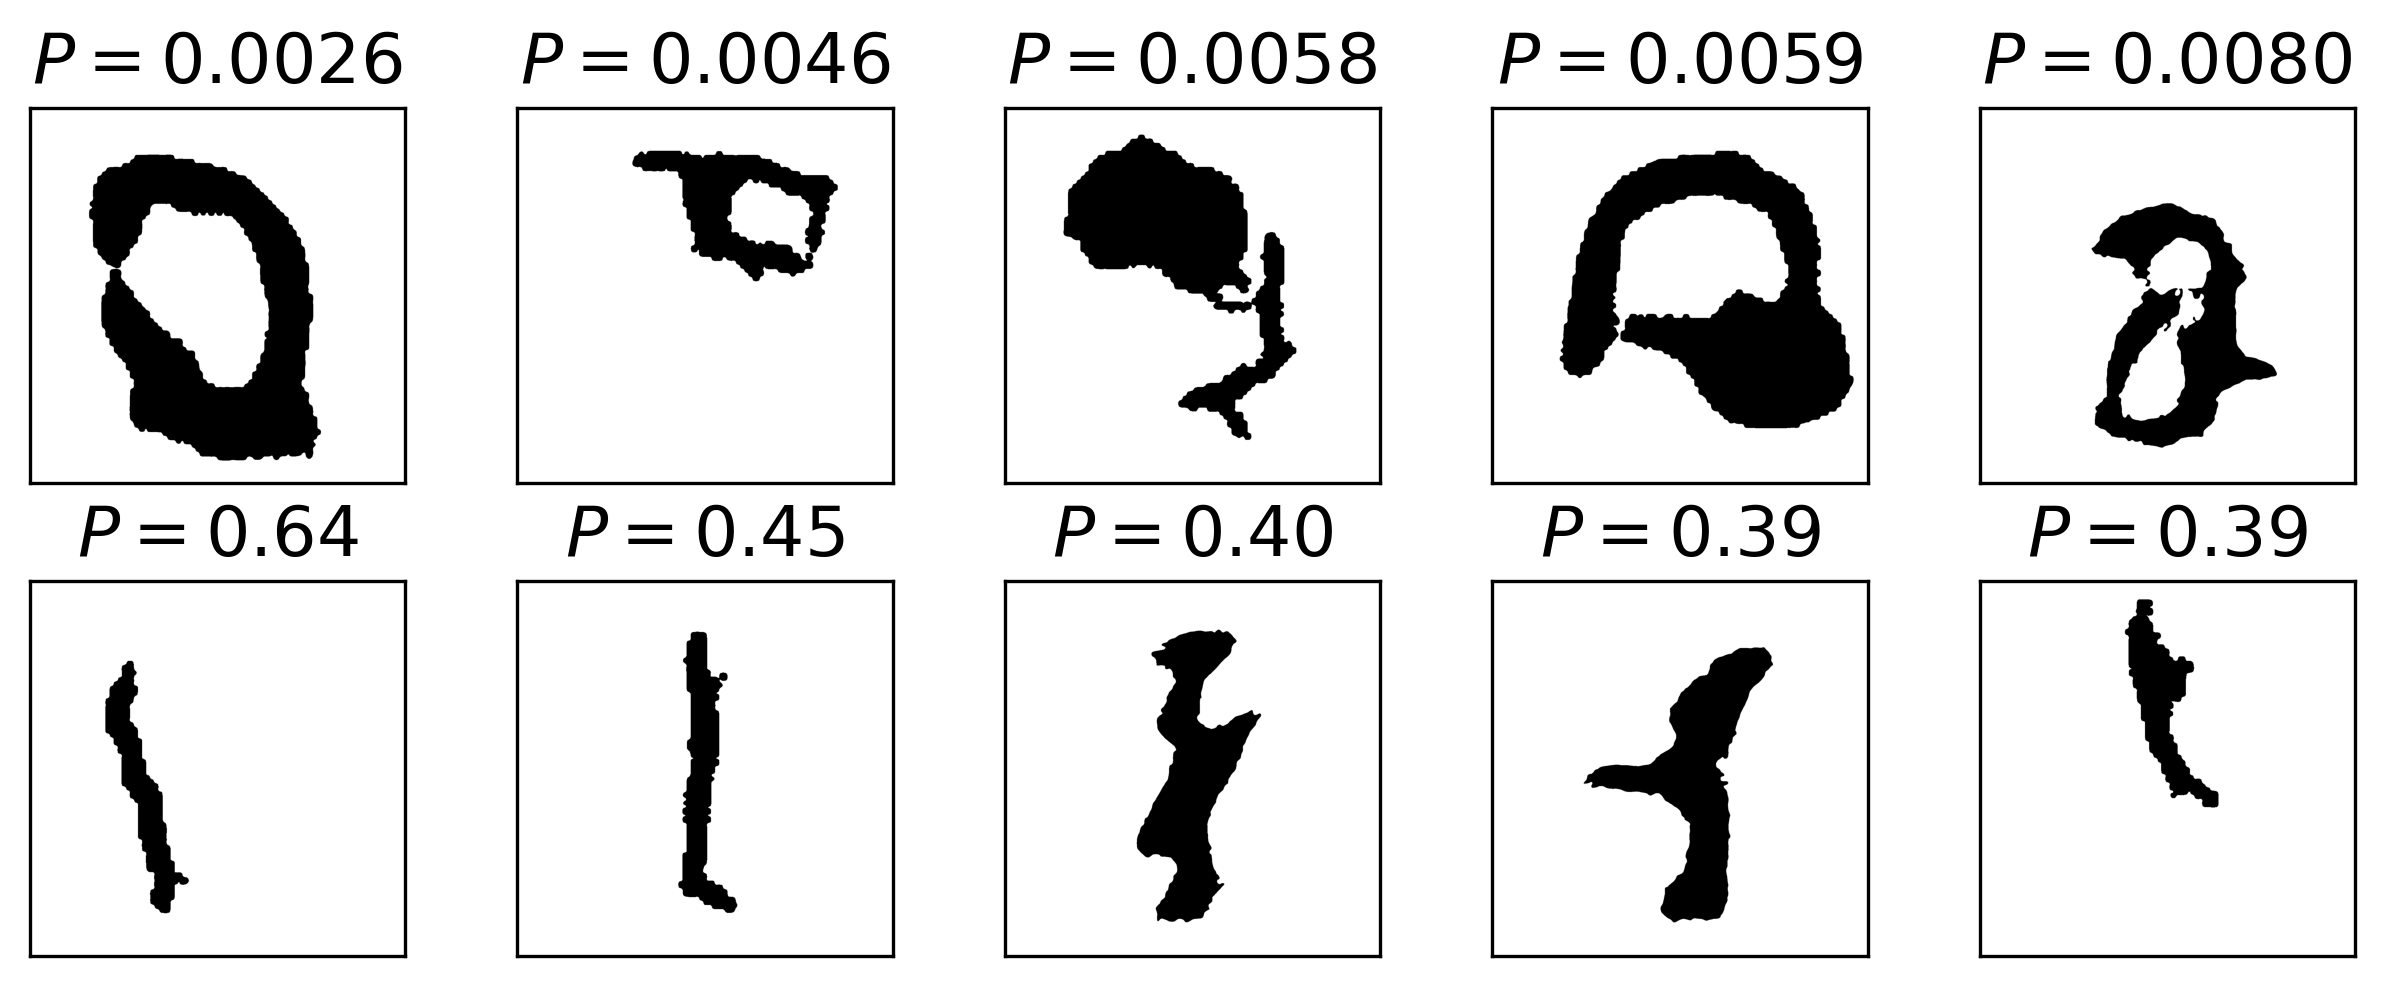
\includegraphics[width=0.4\linewidth]{images/groups-score-0.60.png}
    \label{fig:small-gap}}
  \hfill
  \subfigure[$0.65 \le C < 0.75$]{
    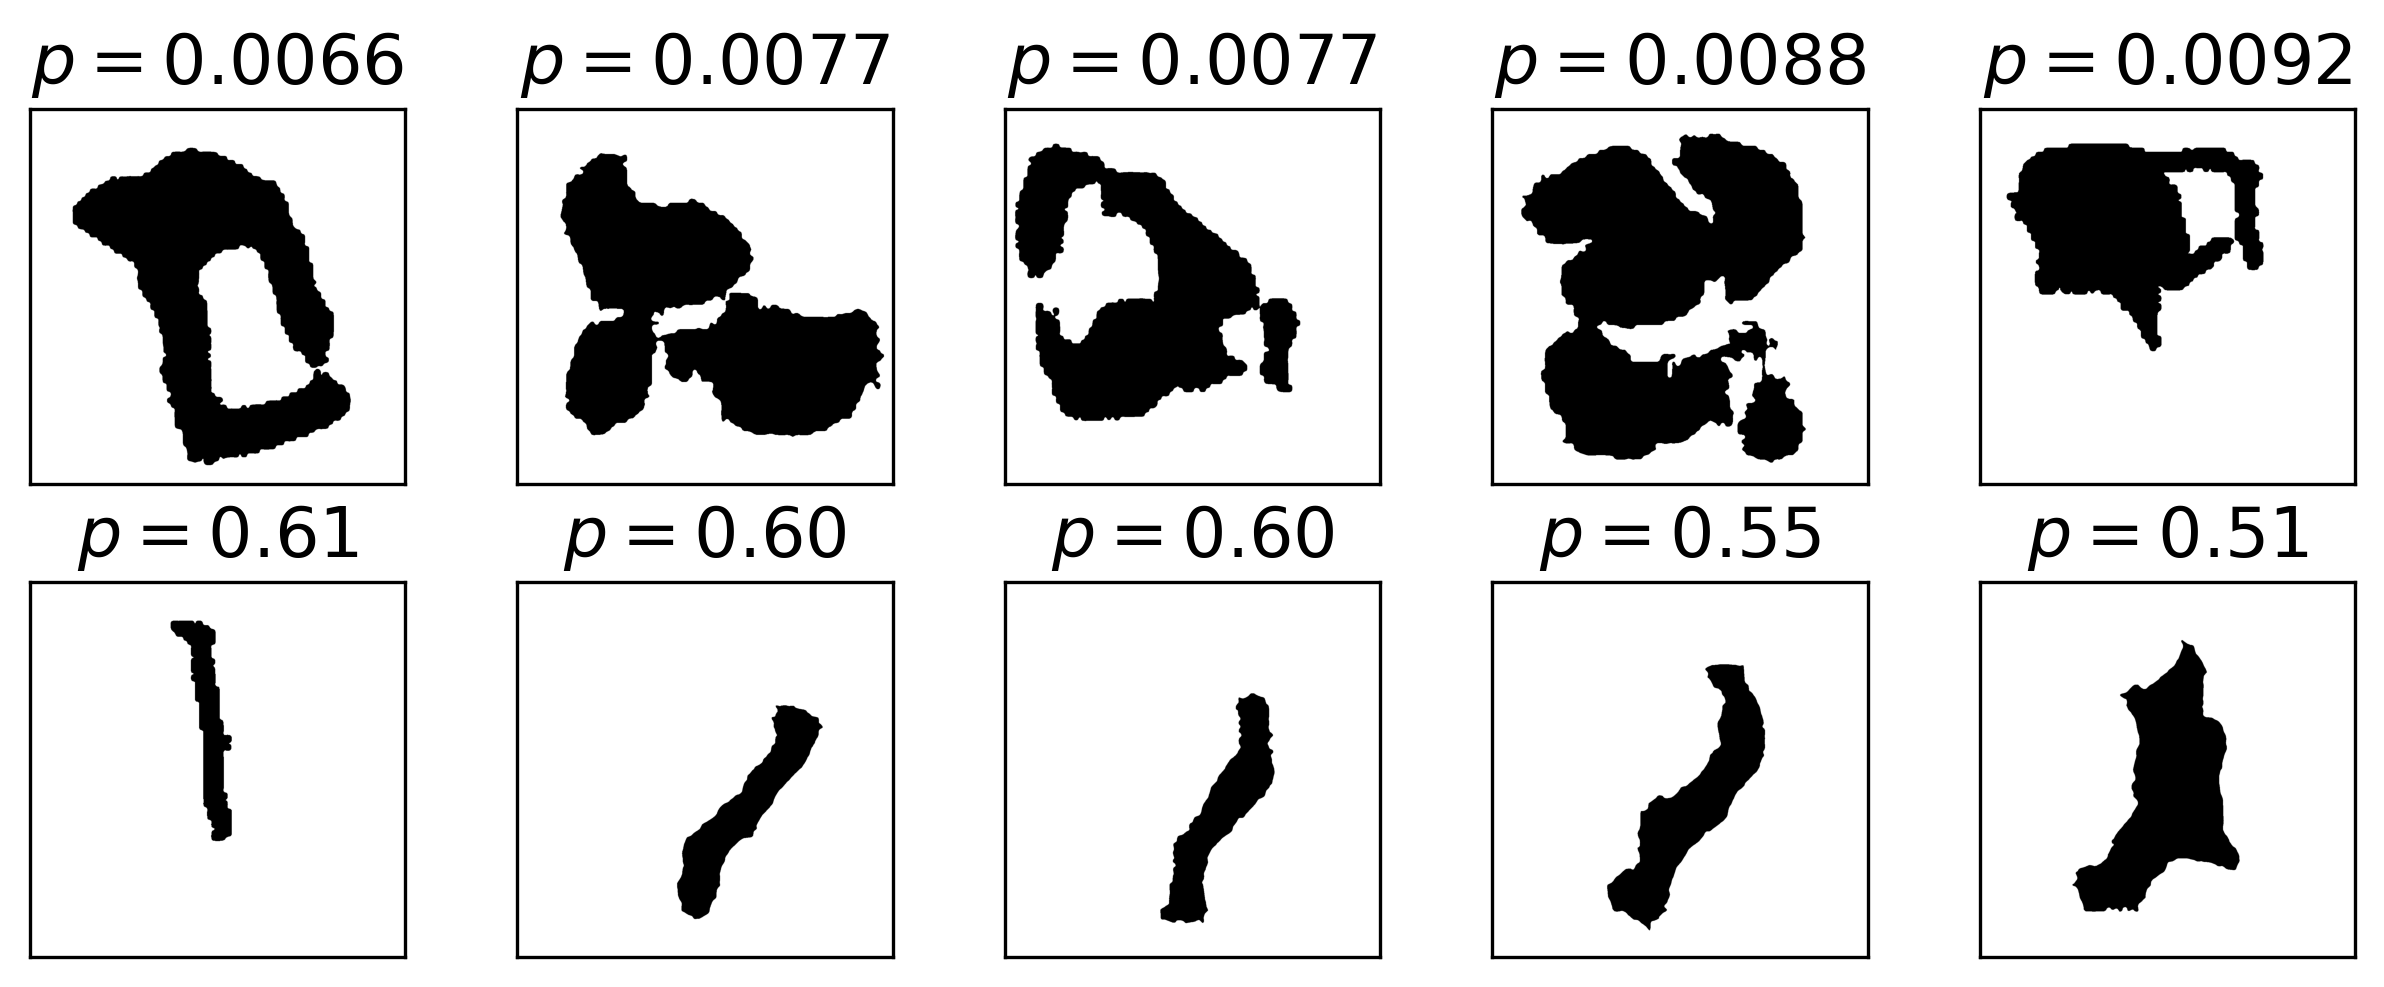
\includegraphics[width=0.4\linewidth]{images/groups-score-0.70.png}}
  \vskip\baselineskip
  \subfigure[$0.75 \le C < 0.85$]{
    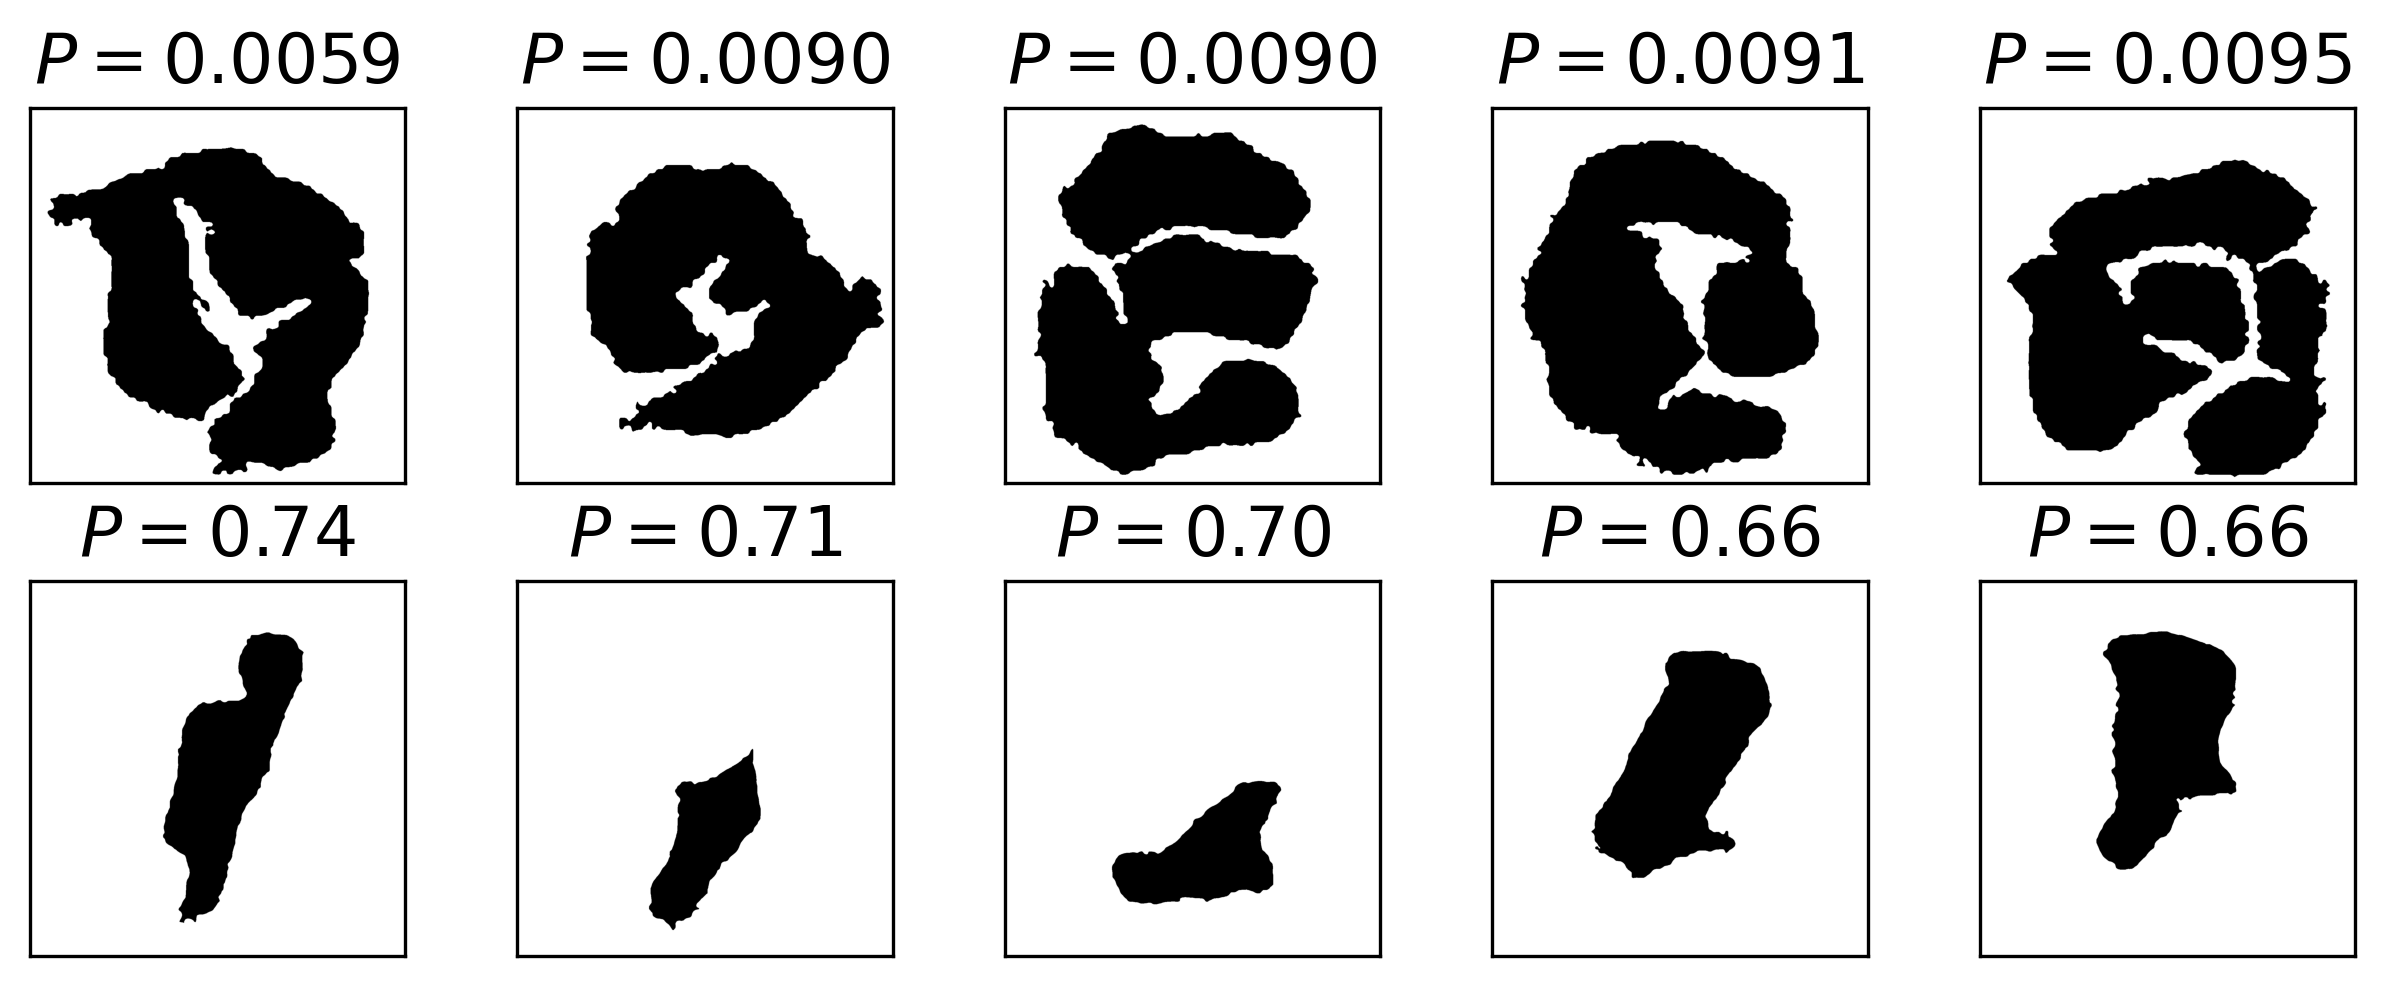
\includegraphics[width=0.4\linewidth]{images/groups-score-0.80.png}}
  \hfill
  \subfigure[$0.85 \le C < 0.95$]{
    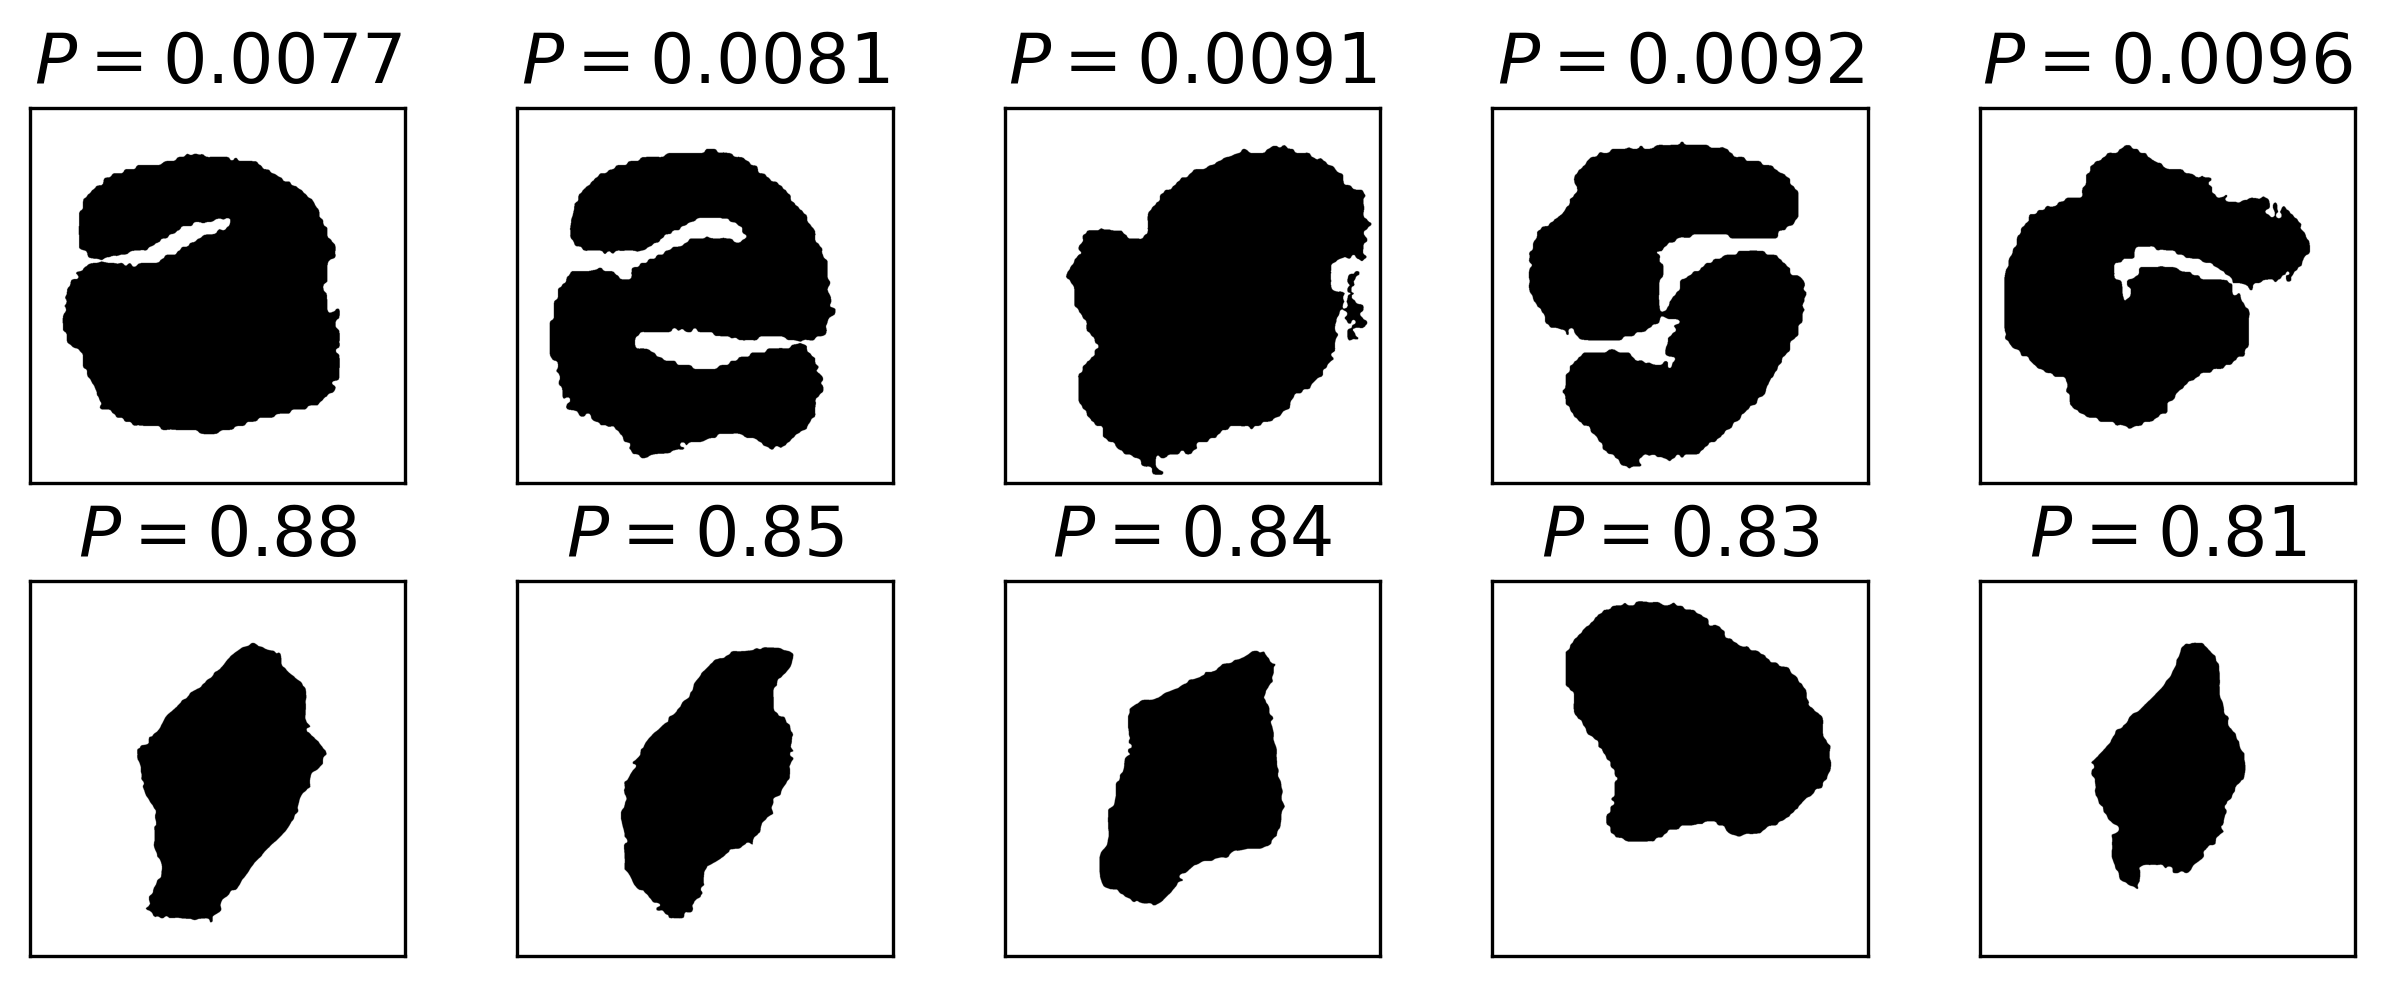
\includegraphics[width=0.4\linewidth]{images/groups-score-0.90.png}
    \label{fig:small-blob}}
  \caption[]{Pores divided into groups by their convexity. Upper row of each
    subfigure: pores with minimal \highlight{awesomeness} in the group, lower
    row: pores with maximal \highlight{awesomeness} in the group.}
  \label{fig:convexity-groups-score}
\end{figure*}

\begin{figure*}
  \centering
  \subfigure[$0.55 \le C < 0.65$]{
    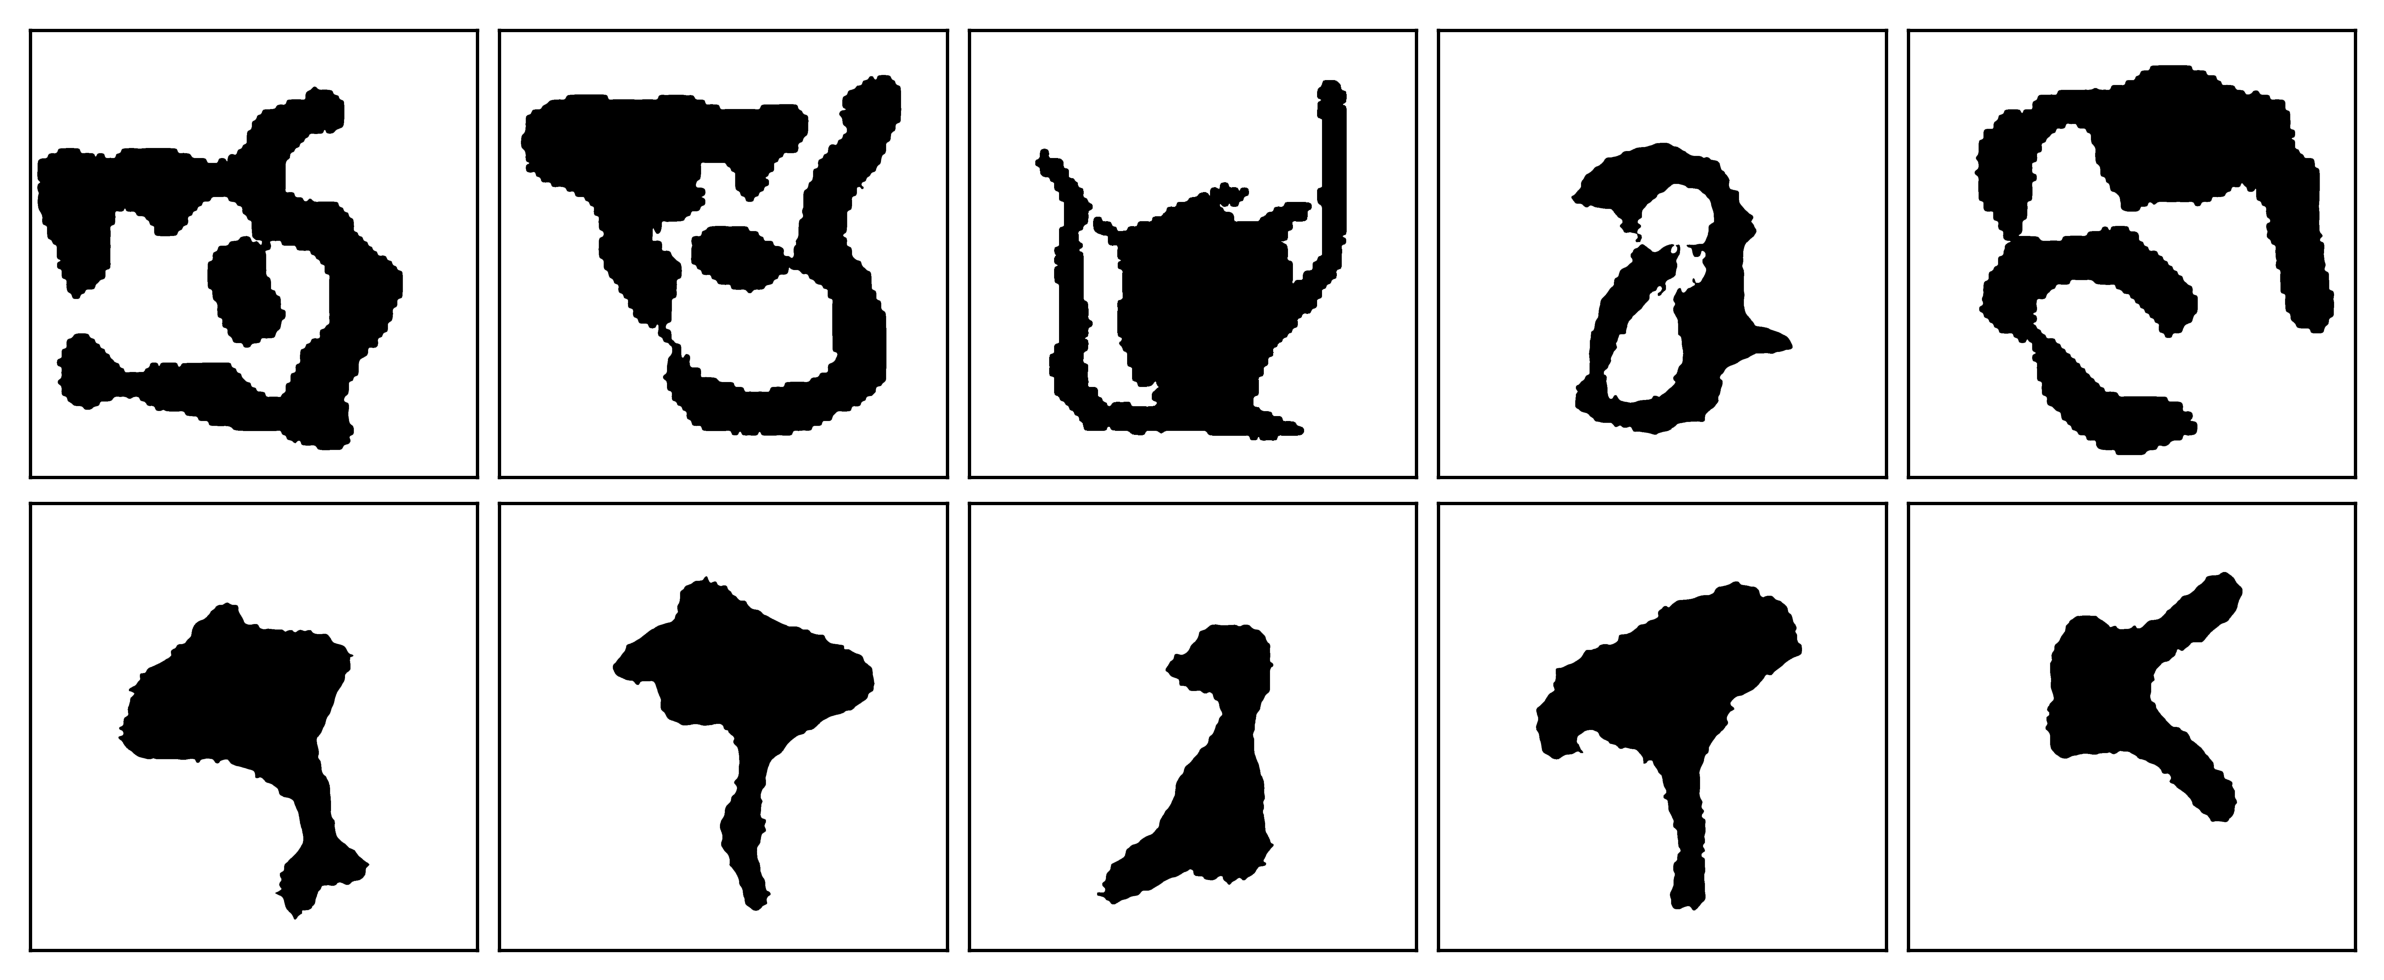
\includegraphics[width=0.4\linewidth]{images/groups-sphericity-0.60.png}}
  \hfill
  \subfigure[$0.65 \le C < 0.75$]{
    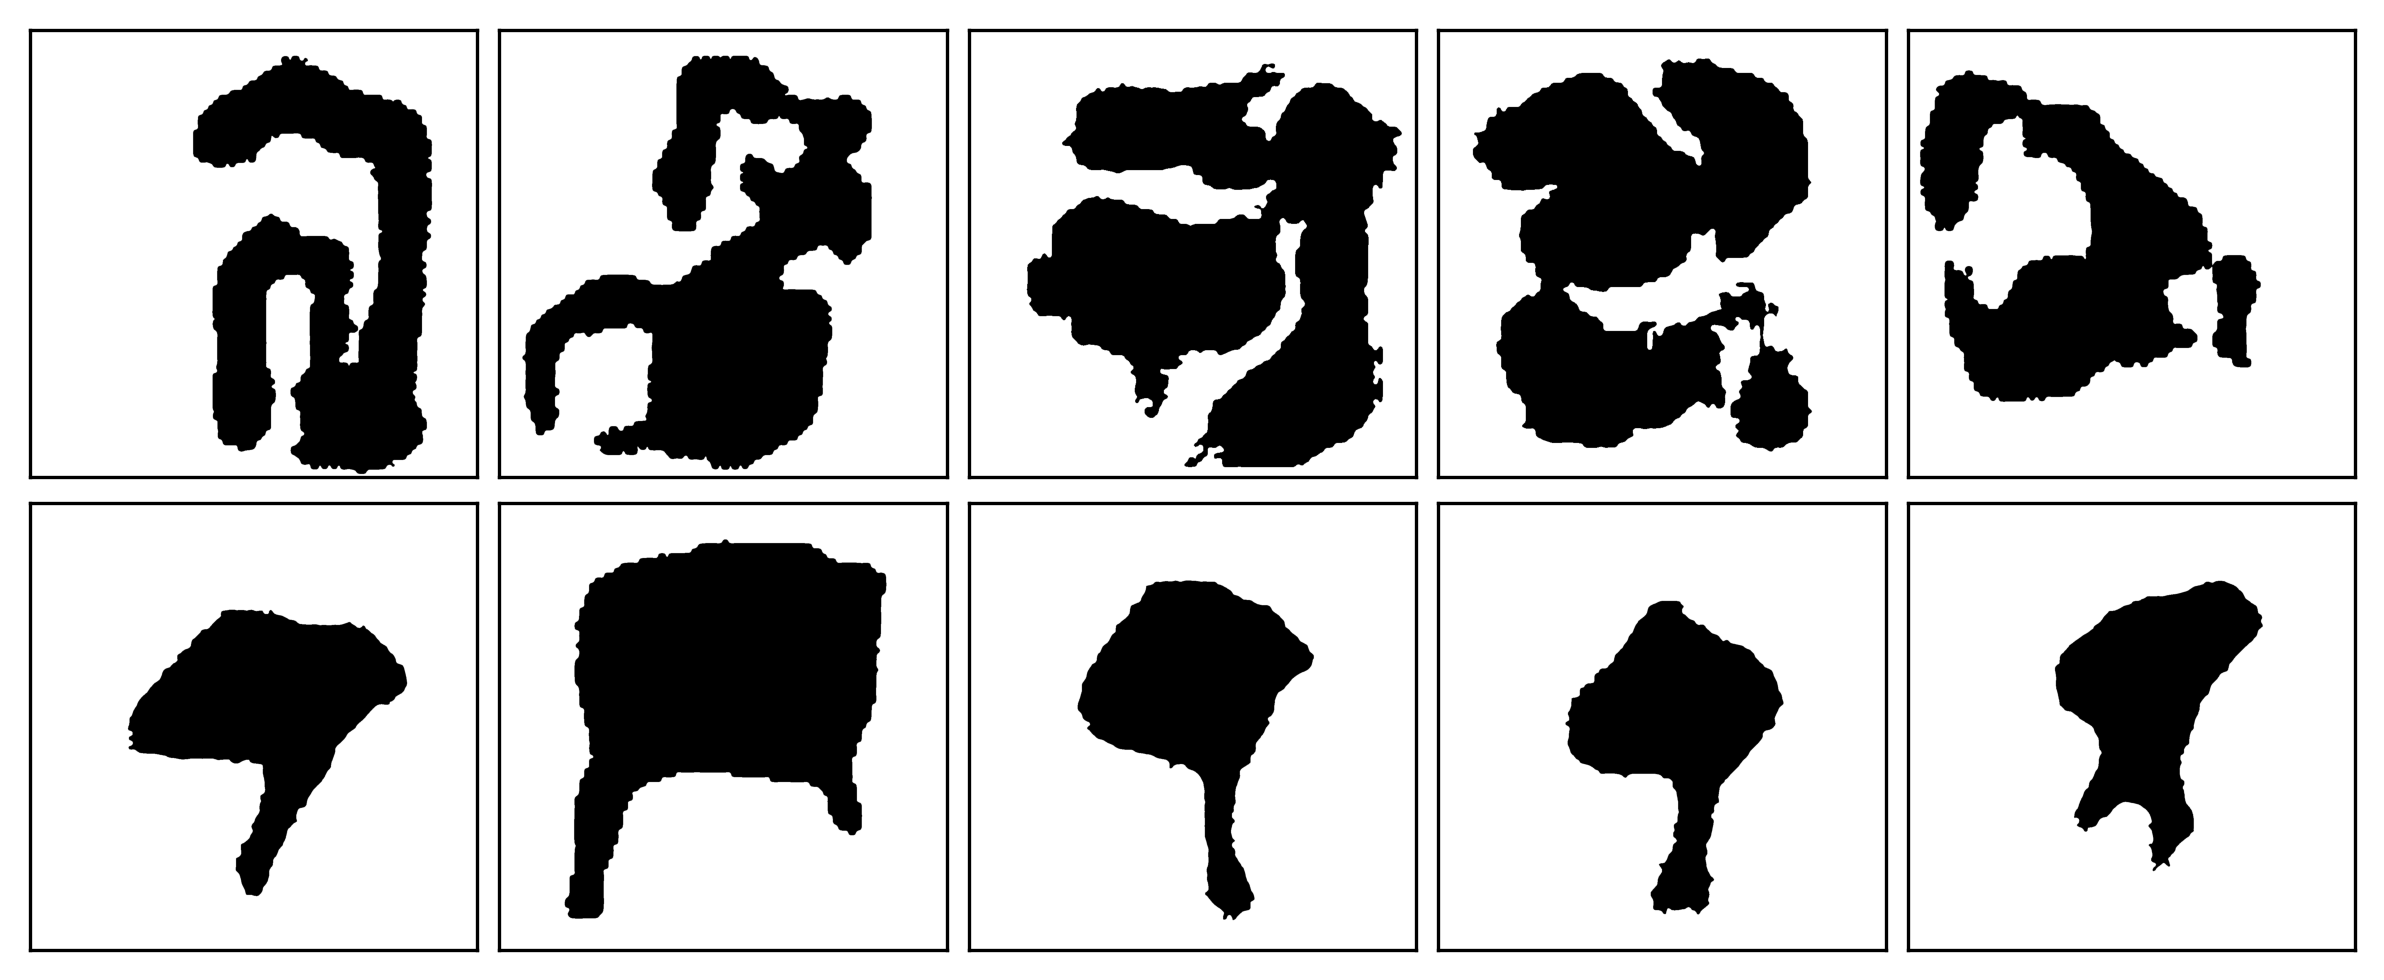
\includegraphics[width=0.4\linewidth]{images/groups-sphericity-0.70.png}}
  \vskip\baselineskip
  \subfigure[$0.75 \le C < 0.85$]{
    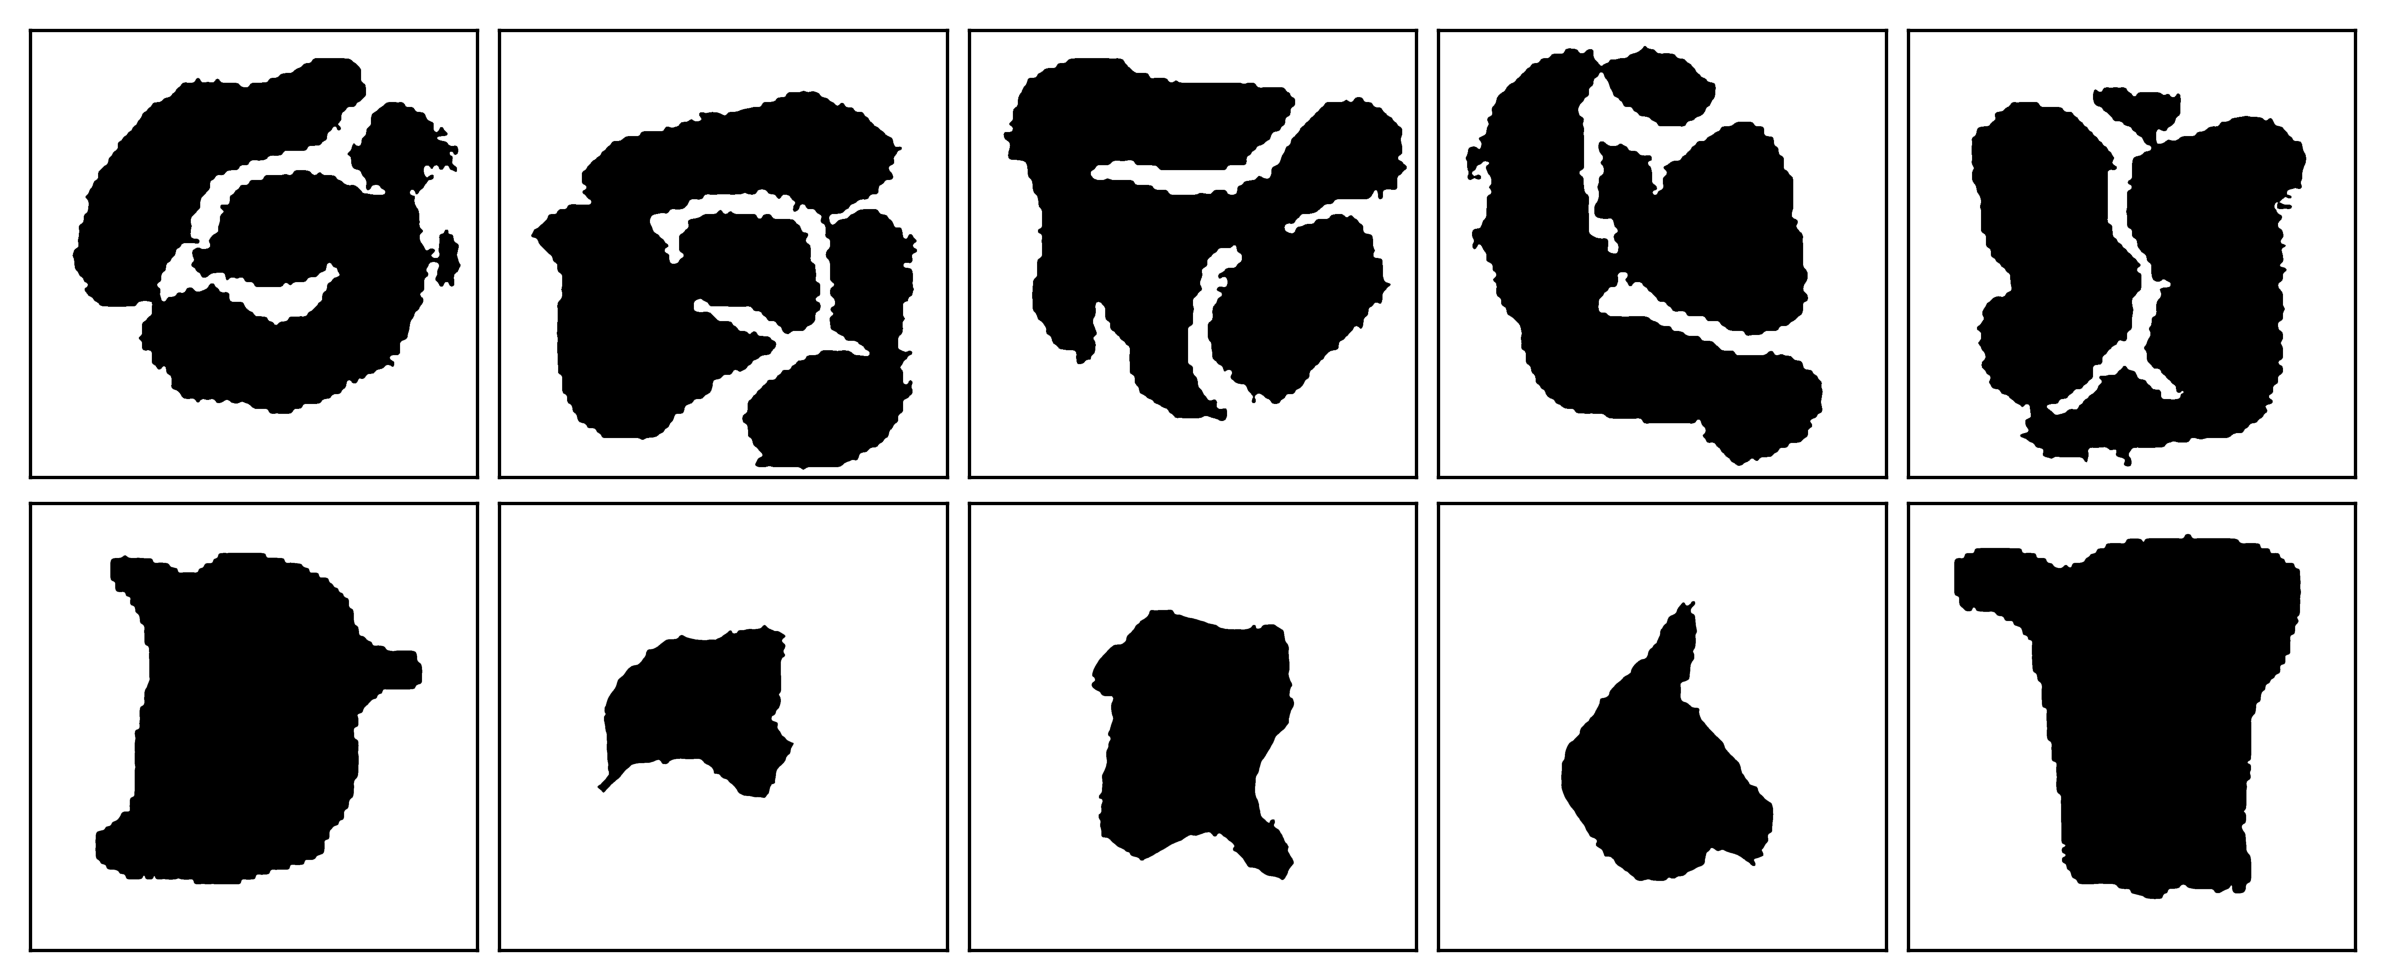
\includegraphics[width=0.4\linewidth]{images/groups-sphericity-0.80.png}}
  \hfill
  \subfigure[$0.85 \le C < 0.95$]{
    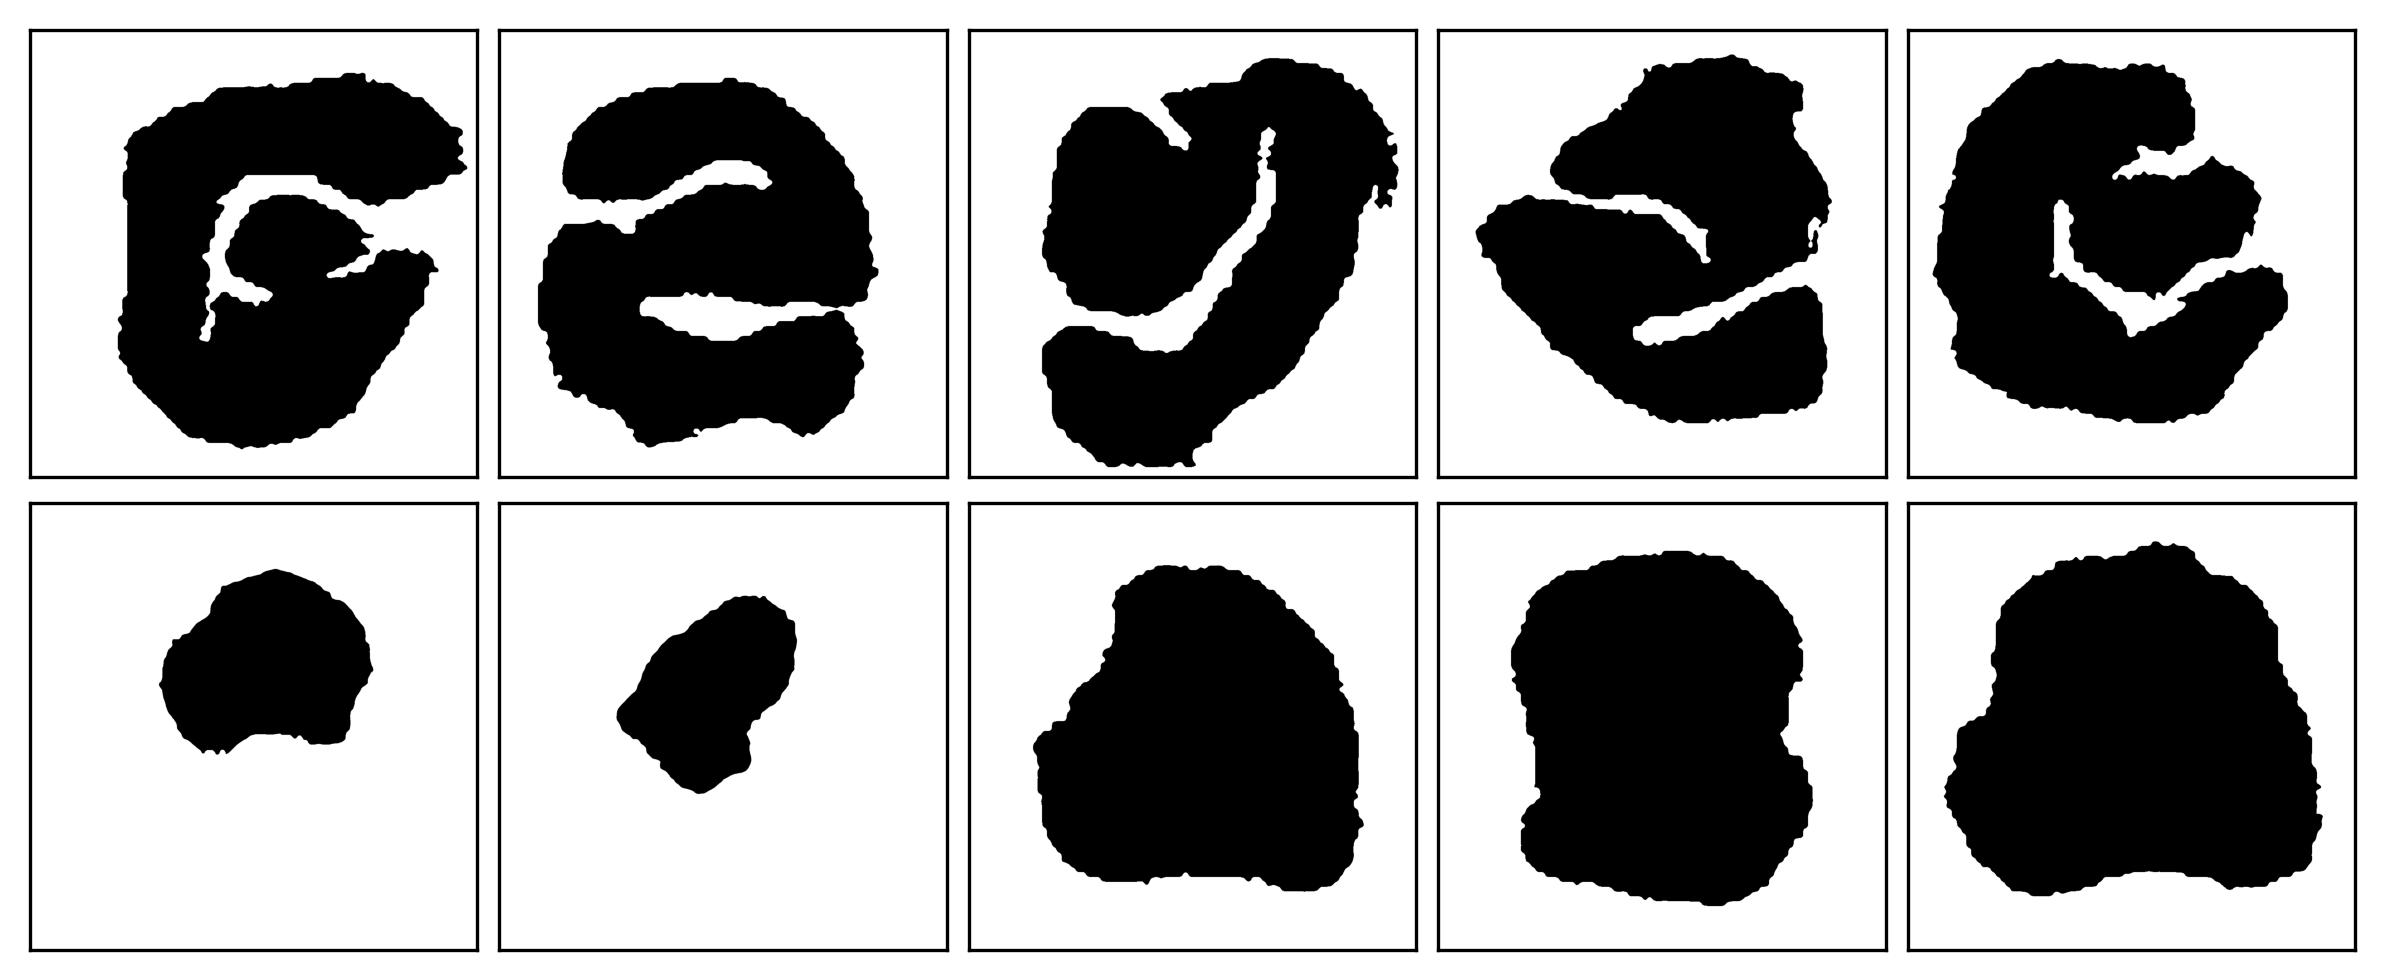
\includegraphics[width=0.4\linewidth]{images/groups-sphericity-0.90.png}}
  \caption[]{Pores divided into groups by their convexity. Upper row of each
    subfigure: pores with minimal roundness in the group, lower row: pores with
    maximal roundness in the group.}
  \label{fig:convexity-groups-roundness}
\end{figure*}

\section{Summary}
In this paper we have developed a new parameter for assession of pore
clusterization quality which can be used as a replacement for roundness
parameter. Benefits of this parameter include:
\begin{itemize}
\item Lower absoulute value of correlation with other common parameters, such as
  convexity, elongation and roundness.
\item Ease of computation and interpretation.
\item Ability to precisely separate well-clusterized pores and underclusterized
  pores in a high convexity range, even if roundness fails to do so.
\item Rotation and resize invariance.
\end{itemize}

Flaws of this parameter include:
\begin{itemize}
\item C-shaped pores with a small gap, like the pore on the left-top of
  \cref{fig:small-gap} always have small \highlight{awesomeness}, even if they
  are otherwise clusterized correctly.
\item Small changes to an image of a pore, when cleverly done, can make drastic
  changes in \highlight{awesomeness}.
\end{itemize}

The first flaw can be dealt with by replacing the Euclidean distance in
\cref{eq:intro} with the length of the shortest path between points which does
not cross the pore's boundary. This, however, can increase computational time
significantly.

The second flaw means that a pore with a very small attachment (compared to the
pore's total surface) connected with a thin throat to the pore's main body has
low \highlight{awesomeness}, like the third pore on \cref{fig:small-blob}, a row
on the top. Normally, small attachments like this do not contribute to any
physical process in any way, so they can simply be ignored and, therefore, their
impact on \highlight{awesomeness} may be not justified.

\bibliography{paper}
\end{document}
